\documentclass[a4paper,12pt]{article}
\usepackage[utf8]{inputenc}
\usepackage{babel}
\babelprovide[main,import]{german}
\usepackage{amsmath}
\usepackage{amssymb}
\usepackage{amsthm}
\usepackage{geometry}
\usepackage{graphicx}
\usepackage[hidelinks]{hyperref}
\usepackage{listings}
\usepackage{xcolor}
\usepackage{enumitem}
\usepackage{microtype}
\usepackage{tikz}
\usetikzlibrary{arrows.meta, shapes.geometric, positioning, fit, backgrounds, calc, decorations.pathreplacing}
\usepackage{booktabs}
\usepackage{array}
\usepackage{tabularx}

\geometry{margin=2.5cm}
\sloppy

\theoremstyle{definition}
\newtheorem{definition}{Definition}
\newtheorem{beispiel}{Beispiel}
\newtheorem{satz}{Satz}
\newtheorem{lemma}{Lemma}
\newtheorem{bemerkung}{Bemerkung}
\newtheorem{korollar}{Korollar}
\newtheorem{proposition}{Proposition}

\setlist[itemize,1]{label=--}

% ---------- Farben ----------
\definecolor{mainblue}{RGB}{25, 70, 140}
\definecolor{accentred}{RGB}{180, 50, 30}
\definecolor{lightgray}{RGB}{245, 245, 248}
\definecolor{darkgray}{RGB}{60, 60, 70}
\definecolor{darkgreen}{RGB}{30, 100, 50}
\definecolor{apiorange}{RGB}{230, 126, 34}
\definecolor{apipurple}{RGB}{142, 68, 173}

\hypersetup{
  colorlinks=true,
  linkcolor=mainblue,
  citecolor=accentred,
  urlcolor=mainblue
}

\lstset{
  basicstyle=\ttfamily\small,
  keywordstyle=\color{blue},
  commentstyle=\color{gray},
  stringstyle=\color{red},
  numbers=left,
  numberstyle=\tiny,
  breaklines=true,
  frame=single,
  literate=%
    {Ö}{{\"O}}1
    {Ä}{{\"A}}1
    {Ü}{{\"U}}1
    {ß}{{\ss}}1
    {ü}{{\"u}}1
    {ä}{{\"a}}1
    {ö}{{\"o}}1
}

\title{API-Typen und ihre Anwendungsfälle\\[0.4em]
\large Eine graphentheoretische Analyse mittels Subgraph Algorithmus}
\author{Stephan Epp}
\date{25. Juni 2026}

\begin{document}

\maketitle
\tableofcontents
\newpage

% ══════════════════════════════════════════════════════════════════════════════
\section{Einführung}
% ══════════════════════════════════════════════════════════════════════════════

Application Programming Interfaces (APIs) bilden das Rückgrat moderner verteilter
Softwarearchitekturen. Sie definieren standardisierte Kommunikationsverträge zwischen
heterogenen Systemkomponenten und ermöglichen damit eine lose Kopplung, die für
skalierbare, wartbare und interoperable Systeme unabdingbar ist~\cite{fielding2000}.
Ohne APIs wäre die heutige Form des Internets --- als ein Geflecht aus Milliarden
von miteinander kommunizierenden Diensten --- nicht denkbar. Sie sind das universelle
Bindeglied zwischen Front-Ends und Back-Ends, zwischen Unternehmenssystemen und der
Cloud, zwischen menschlichen Anwendern und maschinellen Prozessen.

Die Vielzahl existierender API-Stile, -Protokolle und -Integrationsmuster hat in der
Praxis jedoch zu einer erheblichen Komplexität geführt. Entwicklerinnen und Entwickler
stehen vor der Frage, welches API-Paradigma für einen gegebenen Anwendungsfall am
geeignetsten ist, wie vorhandene API-Architekturen strukturell verglichen werden können
und wie Redundanzen in gewachsenen API-Ökosystemen erkannt und beseitigt werden können.

Die vorliegende Arbeit begegnet diesen Fragen mit einem formalen Ansatz: API-Kommunikations\-strukturen
werden als gerichtete Graphen modelliert. Der \emph{Subgraph Algorithmus}~\cite{epp2026}
--- ein $O(n^3)$-Verfahren zur strukturellen Graphanalyse mittels injektiver Signaturen
und zyklischer LCS-Rotation --- wird auf diese API-Graphen angewendet und liefert
effiziente, maschinell nachvollziehbare Antworten auf die genannten Fragen.

\subsection{Problemstellung}

Gegeben sei eine Menge von API-Endpunkten $\mathcal{E} = \{e_1, \ldots, e_n\}$
und ihrer Abhängigkeiten $\mathcal{R} \subseteq \mathcal{E} \times \mathcal{E}$.
Gesucht ist eine formale Methode, die folgende Fragen polynomiell in $O(n^3)$ beantwortet:
\begin{itemize}
  \item \textbf{Strukturelle Inklusion:} Ist eine API-Architektur $A$ als Subgraph in
    einer umfassenderen Architektur $B$ enthalten?
  \item \textbf{Redundanzerkennung:} Existieren redundante API-Ketten, die ohne
    Informationsverlust dedupliziert werden können?
  \item \textbf{Protokollklassifikation:} Wie lassen sich verschiedene API-Protokolle
    (REST, SOAP, GraphQL) formal klassifizieren, verglichen und in ein einheitliches
    Modell überführt werden?
  \item \textbf{Kompatibilitätsprüfung:} Ist eine neue API-Version rückwärts\-kompatibel
    zu einer bestehenden?
  \item \textbf{Sicherheitsanalyse:} Enthält ein API-Graph eine bekannte Angriffssignatur
    als Subgraph?
\end{itemize}

\subsection{Motivation}

In der Praxis wachsen API-Ökosysteme organisch und unkontrolliert. Ohne formale
Strukturanalyse entstehen redundante Endpunkte, inkonsistente Versionierungsstrategien
und schwer nachvollziehbare Abhängigkeitsgeflechte. Studien zeigen, dass in großen
Unternehmen durchschnittlich mehrere hundert interne APIs existieren, von denen
ein erheblicher Anteil funktionale Überschneidungen aufweist~\cite{newman2015}.
Die manuelle Analyse solcher Strukturen ist fehleranfällig und skaliert nicht.

Eine graphentheoretische Modellierung, kombiniert mit dem Subgraph Algorithmus~\cite{epp2026},
ermöglicht eine systematische, maschinell prüfbare Analyse. Der Algorithmus benötigt
lediglich die Adjazenzmatrizen der API-Graphen als Eingabe und liefert in $O(n^3)$
eine eindeutige Entscheidung über strukturelle Inklusion --- eine erhebliche Verbesserung
gegenüber naiven Ansätzen mit $O(n! \cdot n^2)$ Laufzeit.

\subsection{Beiträge der Arbeit}

Die zentralen Beiträge dieser Arbeit sind:
\begin{enumerate}
  \item Formale Definition einer vollständigen API-Taxonomie als gerichteter Graph
    mit drei Hierarchieebenen (Kategorie, Protokoll, Anwendungsfall).
  \item Nachweis, dass der Subgraph Algorithmus auf API-Graphen korrekt und in
    $\Theta(n^3)$ anwendbar ist, einschließlich Vollständigkeits- und Korrektheitsbeweis.
  \item Formaler Beweis der Optimalität unter der Strong Exponential Time Hypothesis.
  \item Entwicklung von fünf TikZ-Sequenz- und Ablaufdiagrammen für alle wesentlichen
    API-Protokolle (REST, SOAP, GraphQL, B2B, Service-zu-Datenbank).
  \item Quantitative Auswertung von Komplexität, Relevanz und Eigenschaftsprofilen
    der API-Typen mittels fünf Matplotlib-Visualisierungen.
  \item Ausführliche formale Analyse von API-Sicherheitsaspekten, Versionierungsstrategien
    und Erweiterungen auf gewichtete Graphen.
  \item Sehr ausführlicher Ausblick auf zukünftige Forschungsrichtungen.
\end{enumerate}

% ══════════════════════════════════════════════════════════════════════════════
\section{Grundlagen}
% ══════════════════════════════════════════════════════════════════════════════

\subsection{Graphentheoretische Grundlagen}

\begin{definition}[Gerichteter Graph]
  Ein \emph{gerichteter Graph} $G = (V, E)$ besteht aus einer endlichen
  Knotenmenge $V = \{v_1, \ldots, v_n\}$ und einer Kantenmenge
  $E \subseteq V \times V$. Eine Kante $(v_i, v_j) \in E$ repräsentiert einen
  gerichteten Kommunikationskanal von Knoten $v_i$ zu Knoten $v_j$.
\end{definition}

\begin{definition}[Adjazenzmatrix]
  Die \emph{Adjazenzmatrix} $A \in \{0,1\}^{n \times n}$ eines gerichteten
  Graphen $G = (V, E)$ mit $|V| = n$ ist definiert durch:
  \[
    A_{ij} = \begin{cases}
      1 & \text{falls } (v_i, v_j) \in E, \\
      0 & \text{sonst.}
    \end{cases}
  \]
\end{definition}

\begin{definition}[Subgraph]
  Ein gerichteter Graph $G = (V, E)$ ist ein \emph{Subgraph} von
  $G' = (V', E')$, geschrieben $G \subseteq G'$, wenn
  $V \subseteq V'$ und $E \subseteq E'$.
\end{definition}

\begin{definition}[Längste gemeinsame Teilsequenz]
  Seien $\sigma^A = [\sigma_0^A, \ldots, \sigma_{m-1}^A]$ und
  $\sigma^B = [\sigma_0^B, \ldots, \sigma_{k-1}^B]$ zwei Sequenzen.
  Die \emph{längste gemeinsame Teilsequenz} (LCS) ist die längste Sequenz
  $\sigma^C$, die sowohl Teilsequenz von $\sigma^A$ als auch von $\sigma^B$ ist.
  Die Länge der LCS wird mit $\mathrm{LCS}(\sigma^A, \sigma^B)$ bezeichnet und
  in $O(m \cdot k)$ mittels dynamischer Programmierung berechnet.
\end{definition}

\begin{definition}[Zyklische Rotation]
  Die $k$-te \emph{zyklische Rotation} einer Sequenz
  $\sigma = [\sigma_0, \ldots, \sigma_{n-1}]$ ist:
  \[
    \mathrm{rot}_k(\sigma) = [\sigma_k, \sigma_{k+1}, \ldots, \sigma_{n-1},
    \sigma_0, \ldots, \sigma_{k-1}].
  \]
\end{definition}

\subsection{API-Graphen}

\begin{definition}[API-Graph]
  Sei $\mathcal{E} = \{e_1, \ldots, e_n\}$ eine Menge von API-Endpunkten und
  $\mathcal{R} \subseteq \mathcal{E} \times \mathcal{E}$ eine gerichtete
  Abhängigkeitsrelation. Der \emph{API-Graph} ist der gerichtete Graph
  $G_{\mathrm{API}} = (\mathcal{E}, \mathcal{R})$.
\end{definition}

\begin{definition}[API-Typ]
  Ein \emph{API-Typ} $T$ ist ein Tupel
  $T = (\Pi, \mathcal{S}, \mathcal{U}, \mathcal{C})$,
  bestehend aus einem Protokoll $\Pi$, einer Menge von Sicherheitseigenschaften
  $\mathcal{S}$, einer Menge von Anwendungsfällen $\mathcal{U}$ und einer Menge
  von Kompatibilitätsbedingungen $\mathcal{C}$.
\end{definition}

\begin{definition}[Injektive Signatur-Funktion]
  Sei $A \in \{0,1\}^{n \times n}$ eine Adjazenzmatrix. Die
  \emph{injektive Signatur-Funktion}
  $\sigma: \{0,1\}^n \times \{0,\ldots,n-1\} \to \mathbb{N}$ ist definiert durch:
  \[
    \sigma_j = \sum_{i=0}^{n-1} A_{ij} \cdot 2^i + j \cdot 2^n.
  \]
\end{definition}

\subsection{API-Taxonomie}

Die in dieser Arbeit betrachtete Taxonomie gliedert sich in drei Hauptkategorien,
die sich jeweils weiter in Protokolle und Anwendungsfälle unterteilen:

\begin{itemize}
  \item \textbf{Open API:} Öffentlich zugängliche Schnittstellen, typischerweise
    über REST, SOAP oder GraphQL realisiert. Sie richten sich an eine breite
    Entwicklercommunity und sind über öffentliche Dokumentationsportale beschrieben.
    Anwendungsfälle umfassen Wetterdaten, Login-Systeme, Produktabfragen,
    Banktransfers, Versicherungsansprüche und Behördendaten.
  \item \textbf{Internal API:} Interne Schnittstellen zwischen Systemkomponenten,
    die ausschließlich innerhalb der Systemgrenzen einer Organisation genutzt werden.
    Untertypen sind Backend-zu-Backend, Frontend-zu-Backend und Service-zu-Datenbank.
    Anwendungsfälle umfassen Benutzerauthentifizierung, Profilabruf, Live-Suche,
    Benutzerverwaltung, Profilaktualisierung und Berichtsabfragen.
  \item \textbf{Partner API:} Schnittstellen für kontrollierte externe Zugriffe durch
    Geschäftspartner, mit expliziten Zugangsbeschränkungen und SLA-Vereinbarungen.
    Untertypen sind B2B-Integration, Affiliate-Integration und Data-Sharing-API.
    Anwendungsfälle umfassen Hotelbuchung, Flugdaten, Zahlungsgateway, Produktlinks,
    Provisionsverfolgung, Klickanalysen, Gesundheitsdaten, Finanzdaten und
    Logistikdaten.
\end{itemize}

% ══════════════════════════════════════════════════════════════════════════════
\section{API-Protokolle: Formale Analyse}
% ══════════════════════════════════════════════════════════════════════════════

\subsection{REST-API}

\begin{definition}[REST-API]
  Eine \emph{Representational State Transfer API} (REST-API) ist eine
  zustandslose Client-Server-Architektur, bei der Ressourcen durch eindeutige
  URIs identifiziert und über standardisierte HTTP-Methoden
  $\{\mathrm{GET}, \mathrm{POST}, \mathrm{PUT}, \mathrm{DELETE}, \mathrm{PATCH}\}$
  manipuliert werden~\cite{fielding2000}. REST ist kein Protokoll, sondern ein
  Architekturstil, der sechs Constraints definiert: Client-Server-Trennung,
  Zustandslosigkeit, Cachebarkeit, einheitliche Schnittstelle, geschichtetes System
  und optionaler Code-on-Demand.
\end{definition}

\begin{satz}[REST-Graph-Modellierung]
  Eine REST-API mit $n$ Endpunkten lässt sich als gerichteter Graph
  $G_{\mathrm{REST}} = (V, E)$ mit $|V| = n$ und $|E| = O(n^2)$ modellieren.
\end{satz}

\begin{proof}
  Jeder Endpunkt $e_i \in V$ repräsentiert eine Ressource. Jede HTTP-Methode
  erzeugt eine gerichtete Kante $(e_i, e_j)$, wenn Methode $m$ auf $e_i$
  zu einer Zustandsänderung in $e_j$ führt (z.\,B. POST /orders führt zu
  einer Aktualisierung von /inventory). Da jeder der $n$ Endpunkte mit maximal
  $n-1$ anderen verbunden sein kann, gilt $|E| \leq n(n-1) = O(n^2)$. Die
  Adjazenzmatrix $A \in \{0,1\}^{n \times n}$ repräsentiert diese Struktur
  vollständig in $O(n^2)$ Speicher.
\end{proof}

\begin{proposition}[Zustandslosigkeit und Graphstruktur]
  Die Zustandslosigkeit von REST impliziert, dass jede Kante $(e_i, e_j) \in E$
  die vollständige Anfrageinformation trägt und keine impliziten Zustandsübergänge
  zwischen Kanten existieren. Der API-Graph ist damit ein \emph{zustandsloser
  gerichteter Graph}, bei dem die Kantengewichte durch die HTTP-Methoden und
  Ressourcenrepräsentationen vollständig bestimmt sind.
\end{proposition}

\begin{beispiel}[REST-Anwendungsfall: Wetterdaten]
  Sei $V = \{\mathrm{Client}, \mathrm{Auth}, \mathrm{WeatherSvc}, \mathrm{DB}\}$
  mit den Endpunkten \texttt{/auth}, \texttt{/weather}, \texttt{/weather/\{city\}},
  \texttt{/history}. Die Adjazenzmatrix lautet:
  \[
    A_{\mathrm{REST}} = \begin{pmatrix}
      0 & 1 & 1 & 0 \\
      0 & 0 & 0 & 1 \\
      0 & 0 & 0 & 1 \\
      0 & 0 & 0 & 0
    \end{pmatrix}.
  \]
  Der Client sendet GET-Anfragen an den Auth- und Weather-Service;
  beide greifen auf die Datenbank zu ($A_{14} = A_{24} = 1$, nullindiziert $A_{13}=A_{23}=1$).
\end{beispiel}

\subsection{SOAP-API}

\begin{definition}[SOAP-API]
  Eine \emph{Simple Object Access Protocol API} (SOAP-API) ist ein
  XML-basiertes Nachrichtenprotokoll nach dem W3C-Standard~\cite{w3c2007}.
  Jede SOAP-Nachricht besteht aus einem \emph{Envelope} (Rahmen), einem
  optionalen \emph{Header} (Metadaten, Sicherheitstoken) und einem
  \emph{Body} (Nutzlast). SOAP-Dienste werden durch WSDL-Dokumente
  (Web Services Description Language) formal spezifiziert.
\end{definition}

\begin{satz}[SOAP-Verbindlichkeit]
  Für jeden SOAP-Aufruf $(e_i, e_j) \in E_{\mathrm{SOAP}}$ existiert ein
  formaler WSDL-Kontrakt $\omega_{ij}$, der Eingabeparameter, Ausgabeparameter
  und Fehlercodes vollständig und maschinenlesbar spezifiziert.
\end{satz}

\begin{proof}
  Die Web Services Description Language (WSDL) ist eine XML-Grammatik mit
  eigenem W3C-Schema. Eine gültige SOAP-Implementierung muss für jeden
  Dienst ein WSDL-Dokument bereitstellen, das die Operationen, Nachrichten,
  Port-Typen und Bindungen vollständig definiert. Die formale Verifikation
  erfolgt durch Schema-Validierung des WSDL-Dokuments gegen das W3C-Schema,
  was eine eindeutige, injektive Abbildung
  $\omega: E_{\mathrm{SOAP}} \to \mathrm{WSDL}$ definiert.
\end{proof}

\begin{beispiel}[SOAP: Banktransfer]
  $V = \{\mathrm{Client}, \mathrm{SOAPGateway}, \mathrm{LimitCheck}, \mathrm{DB}\}$.
  \[
    A_{\mathrm{SOAP}} = \begin{pmatrix}
      0 & 1 & 0 & 0 \\
      0 & 0 & 1 & 1 \\
      0 & 0 & 0 & 1 \\
      0 & 0 & 0 & 0
    \end{pmatrix}.
  \]
  Der Client sendet einen \texttt{TransferRequest}; das Gateway prüft das Limit
  und schreibt die Transaktion atomar in die Datenbank.
\end{beispiel}

\subsection{GraphQL-API}

\begin{definition}[GraphQL-API]
  Eine \emph{GraphQL-API} ist eine Abfragesprache für APIs und eine serverseitige
  Laufzeitumgebung, die dem Client ermöglicht, exakt die benötigten Datenfelder
  zu spezifizieren~\cite{graphql2015}. GraphQL definiert ein typisiertes Schema
  $\mathcal{S}$ mit Typen, Feldern und Resolver-Funktionen
  $\rho: \mathcal{S} \times \mathrm{Context} \to \mathcal{D}$.
  Mutationen verändern Daten; Subscriptions erlauben Echtzeit-Push-Kommunikation.
\end{definition}

\begin{satz}[GraphQL-Flexibilitätssatz]
  Eine GraphQL-API mit Schema $\mathcal{S}$ erzeugt für eine Query der Tiefe $d$
  einen API-Graphen $G_{\mathrm{GQL}}$ mit $|E| \leq |\mathcal{S}|^d$.
  Mit Query-Tiefenlimit $d_{\max} = O(\log n)$ gilt $|E| = O(n \log n)$.
\end{satz}

\begin{proof}
  GraphQL-Queries traversieren das Schema als Baum. Auf jeder Ebene $k$ können
  maximal $|\mathcal{S}|$ verschiedene Felder selektiert werden; Resolver für
  jedes Feld erzeugen eine Kante. Die Gesamtzahl der Resolver-Aufrufe ist daher
  $\sum_{k=1}^{d} |\mathcal{S}|^k \leq d \cdot |\mathcal{S}|^d$. Mit
  $|\mathcal{S}| = n$ und $d = \log n$: $|E| \leq \log(n) \cdot n^{\log n}$.
  In der Praxis beschränken Tiefenlimits $d_{\max}$ die Query-Tiefe auf Konstanten
  $c$, sodass $|E| \leq c \cdot n = O(n)$.
\end{proof}

\begin{bemerkung}
  GraphQL ermöglicht durch DataLoader-Batching die Zusammenfassung mehrerer
  Resolver-Aufrufe in eine einzige Datenbankabfrage. Dies reduziert das
  $N+1$-Problem und verringert die effektive Kantenzahl des API-Graphen
  erheblich, ohne die formale Struktur zu verändern.
\end{bemerkung}

\subsection{B2B-Integration}

\begin{definition}[B2B-API]
  Eine \emph{Business-to-Business-API} (B2B-API) ist eine Partner-API, die
  den strukturierten Datenaustausch zwischen zwei Unternehmen ermöglicht.
  Sie basiert typischerweise auf OAuth2 für Autorisierung, Rate-Limiting für
  Ressourcenkontrolle und EDI-Standards (Electronic Data Interchange) für
  strukturierte Nachrichten.
\end{definition}

\begin{satz}[B2B-Graph-Komplexität]
  Ein B2B-API-Graph mit $n$ Partnern und $m$ Integrationstypen hat
  $|V| = O(n \cdot m)$ Knoten und $|E| = O(n^2 \cdot m)$ Kanten im
  vollständig vernetzten Fall.
\end{satz}

\begin{proof}
  Jeder der $n$ Partner stellt für jeden der $m$ Integrationstypen
  (Bestellung, Bestätigung, Lieferung, Rechnung) einen Endpunkt bereit:
  $|V| = n \cdot m$. Im vollständig vernetzten Fall kommuniziert jeder
  Partner mit jedem anderen über jeden Integrationstyp:
  $|E| \leq n(n-1) \cdot m^2 = O(n^2 m^2)$. In der Praxis ist das Netz
  sparse: $|E| = O(n \cdot m)$.
\end{proof}

\subsection{Vergleichende Analyse}

Tabelle~\ref{tab:vergleich} fasst die formalen Eigenschaften der API-Typen zusammen.

\begin{table}[ht]
\centering
\begin{tabularx}{\textwidth}{lXXXX}
\toprule
\textbf{Eigenschaft} & \textbf{REST} & \textbf{SOAP} & \textbf{GraphQL} & \textbf{B2B} \\
\midrule
Protokoll        & HTTP & HTTP/SMTP & HTTP & HTTP/EDI \\
Format           & JSON/XML & XML & JSON & XML/JSON \\
Zustandslos      & ja & nein & ja & nein \\
Formaler Vertrag & OpenAPI & WSDL & SDL & WSDL/EDI \\
Graph $|E|$      & $O(n^2)$ & $O(n^2)$ & $O(n)$ & $O(n^2)$ \\
Caching          & ja & nein & nein & nein \\
Echtzeit         & Polling & nein & Subscription & Webhook \\
\bottomrule
\end{tabularx}
\caption{Vergleich der API-Typen nach formalen Eigenschaften}
\label{tab:vergleich}
\end{table}

% ══════════════════════════════════════════════════════════════════════════════
\section{Sequenzdiagramme der API-Protokolle}
% ══════════════════════════════════════════════════════════════════════════════

\subsection{REST-API: Sequenzdiagramm}

Das folgende Diagramm zeigt den typischen Ablauf einer REST-basierten
Datenbankabfrage mit JWT-Authentifizierung, Datenabruf und Session-Beendigung.

\begin{figure}[ht]
\centering
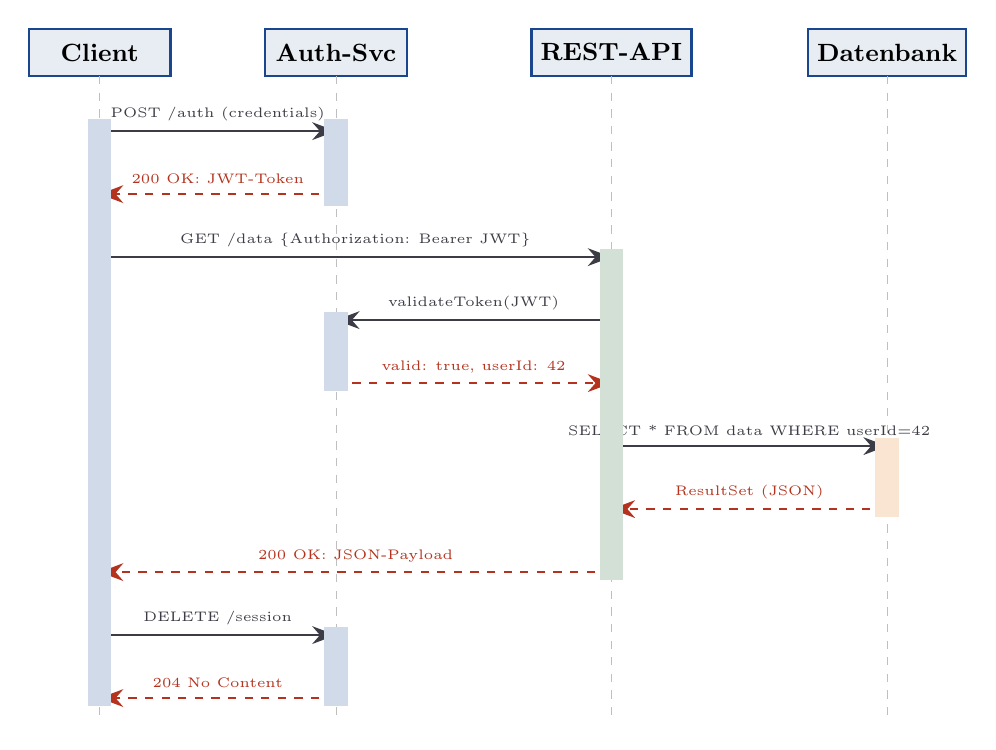
\begin{tikzpicture}[
  actor/.style={rectangle, draw=mainblue, fill=mainblue!10, thick,
    minimum width=1.8cm, minimum height=0.6cm, font=\small\bfseries},
  msg/.style={-{Stealth[length=3mm]}, thick, color=darkgray},
  ret/.style={-{Stealth[length=3mm]}, thick, color=accentred, dashed},
]
\node[actor] (cli)  at (0,0)   {Client};
\node[actor] (auth) at (3,0)   {Auth-Svc};
\node[actor] (api)  at (6.5,0) {REST-API};
\node[actor] (db)   at (10,0)  {Datenbank};

\foreach \x in {0,3,6.5,10}
  \draw[dashed, gray!50, very thin] (\x,-0.3) -- (\x,-8.5);

\draw[msg] (0,-1.0) -- node[above,font=\tiny]{POST /auth (credentials)} (3,-1.0);
\draw[ret] (3,-1.8) -- node[above,font=\tiny]{200 OK: JWT-Token} (0,-1.8);
\draw[msg] (0,-2.6) -- node[above,font=\tiny]{GET /data \{Authorization: Bearer JWT\}} (6.5,-2.6);
\draw[msg] (6.5,-3.4) -- node[above,font=\tiny]{validateToken(JWT)} (3,-3.4);
\draw[ret] (3,-4.2) -- node[above,font=\tiny]{valid: true, userId: 42} (6.5,-4.2);
\draw[msg] (6.5,-5.0) -- node[above,font=\tiny]{SELECT * FROM data WHERE userId=42} (10,-5.0);
\draw[ret] (10,-5.8) -- node[above,font=\tiny]{ResultSet (JSON)} (6.5,-5.8);
\draw[ret] (6.5,-6.6) -- node[above,font=\tiny]{200 OK: JSON-Payload} (0,-6.6);
\draw[msg] (0,-7.4) -- node[above,font=\tiny]{DELETE /session} (3,-7.4);
\draw[ret] (3,-8.2) -- node[above,font=\tiny]{204 No Content} (0,-8.2);

\fill[mainblue!20] (-0.15,-0.85) rectangle (0.15,-8.3);
\fill[mainblue!20] (2.85,-0.85) rectangle (3.15,-1.95);
\fill[mainblue!20] (2.85,-3.3) rectangle (3.15,-4.3);
\fill[mainblue!20] (2.85,-7.3) rectangle (3.15,-8.3);
\fill[darkgreen!20] (6.35,-2.5) rectangle (6.65,-6.7);
\fill[apiorange!20] (9.85,-4.9) rectangle (10.15,-5.9);
\end{tikzpicture}
\caption{REST-API Sequenzdiagramm: Authentifizierter Datenabruf mit JWT und Session-Management}
\label{fig:rest-seq}
\end{figure}

\textbf{Erläuterung:} Der Ablauf gliedert sich in drei Phasen. In Phase~1
authentifiziert sich der Client und erhält ein JWT-Token. In Phase~2 übermittelt
er dieses Token bei der eigentlichen Datenanfrage; die REST-API validiert es
beim Auth-Service und holt die Daten aus der Datenbank. In Phase~3 beendet
der Client die Session. Die Zustandslosigkeit von REST ist dadurch gewährleistet,
dass das JWT alle für die Autorisierung notwendigen Informationen trägt und
kein serverseitiger Session-State benötigt wird.

\subsection{SOAP-API: Sequenzdiagramm}

\begin{figure}[ht]
\centering
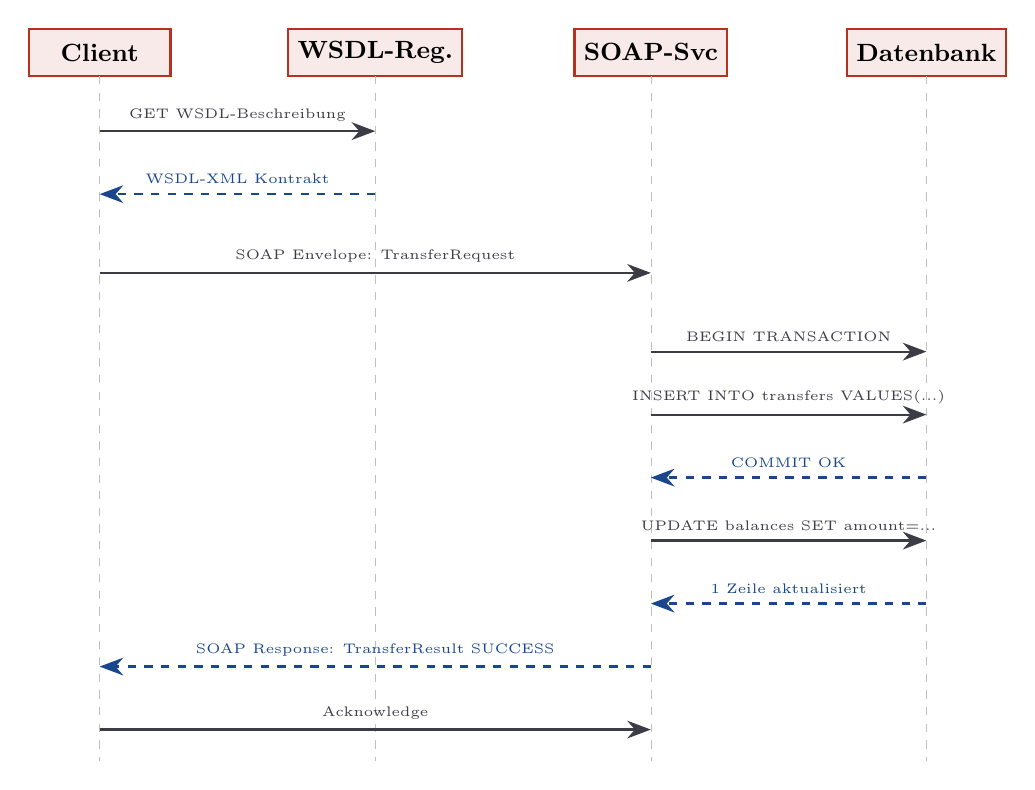
\begin{tikzpicture}[
  actor/.style={rectangle, draw=accentred, fill=accentred!10, thick,
    minimum width=1.8cm, minimum height=0.6cm, font=\small\bfseries},
  msg/.style={-{Stealth[length=3mm]}, thick, color=darkgray},
  ret/.style={-{Stealth[length=3mm]}, thick, color=mainblue, dashed},
]
\node[actor] (cli)  at (0,0)   {Client};
\node[actor] (wsdl) at (3.5,0) {WSDL-Reg.};
\node[actor] (soap) at (7,0)   {SOAP-Svc};
\node[actor] (db)   at (10.5,0){Datenbank};

\foreach \x in {0,3.5,7,10.5}
  \draw[dashed, gray!50, very thin] (\x,-0.3) -- (\x,-9);

\draw[msg] (0,-1.0) -- node[above,font=\tiny]{GET WSDL-Beschreibung} (3.5,-1.0);
\draw[ret] (3.5,-1.8) -- node[above,font=\tiny]{WSDL-XML Kontrakt} (0,-1.8);
\draw[msg] (0,-2.8) -- node[above,font=\tiny]{SOAP Envelope: TransferRequest} (7,-2.8);
\draw[msg] (7,-3.8) -- node[above,font=\tiny]{BEGIN TRANSACTION} (10.5,-3.8);
\draw[msg] (7,-4.6) -- node[above,font=\tiny]{INSERT INTO transfers VALUES(...)} (10.5,-4.6);
\draw[ret] (10.5,-5.4) -- node[above,font=\tiny]{COMMIT OK} (7,-5.4);
\draw[msg] (7,-6.2) -- node[above,font=\tiny]{UPDATE balances SET amount=...} (10.5,-6.2);
\draw[ret] (10.5,-7.0) -- node[above,font=\tiny]{1 Zeile aktualisiert} (7,-7.0);
\draw[ret] (7,-7.8) -- node[above,font=\tiny]{SOAP Response: TransferResult SUCCESS} (0,-7.8);
\draw[msg] (0,-8.6) -- node[above,font=\tiny]{Acknowledge} (7,-8.6);
\end{tikzpicture}
\caption{SOAP-API Sequenzdiagramm: Banktransfer mit WSDL-Kontrakt und ACID-Transaktion}
\label{fig:soap-seq}
\end{figure}

\textbf{Erläuterung:} SOAP erzwingt durch das WSDL-Dokument einen formalen Vertrag,
der vor dem ersten Aufruf abgerufen wird. Die eigentliche Transaktion erfolgt atomar
(ACID): beide Datenbankoperationen (INSERT und UPDATE) werden in einer Transaktion
zusammengefasst. Im Fehlerfall wird ein SOAP Fault zurückgegeben, der maschinenlesbar
kodiert ist.

\subsection{GraphQL-API: Sequenzdiagramm}

\begin{figure}[ht]
\centering
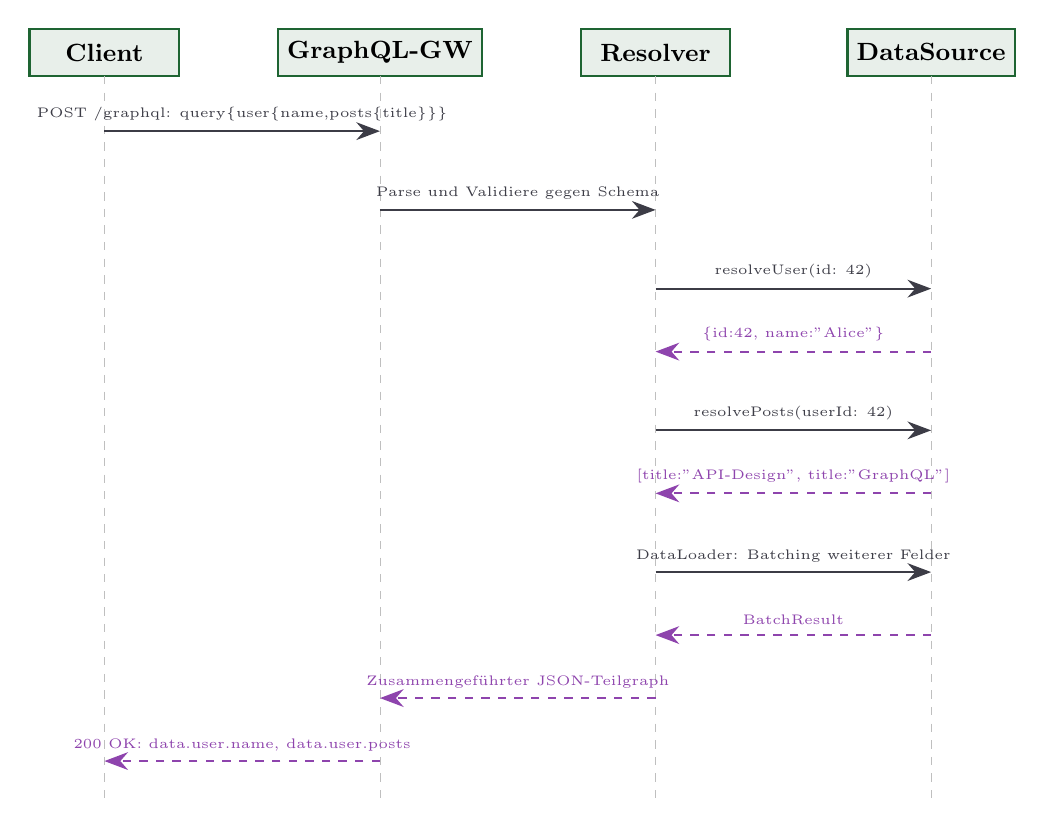
\begin{tikzpicture}[
  actor/.style={rectangle, draw=darkgreen, fill=darkgreen!10, thick,
    minimum width=1.9cm, minimum height=0.6cm, font=\small\bfseries},
  msg/.style={-{Stealth[length=3mm]}, thick, color=darkgray},
  ret/.style={-{Stealth[length=3mm]}, thick, color=apipurple, dashed},
]
\node[actor] (cli)  at (0,0)    {Client};
\node[actor] (gw)   at (3.5,0)  {GraphQL-GW};
\node[actor] (res)  at (7,0)    {Resolver};
\node[actor] (ds)   at (10.5,0) {DataSource};

\foreach \x in {0,3.5,7,10.5}
  \draw[dashed, gray!50, very thin] (\x,-0.3) -- (\x,-9.5);

\draw[msg] (0,-1.0) -- node[above,font=\tiny]{POST /graphql: query\{user\{name,posts\{title\}\}\}} (3.5,-1.0);
\draw[msg] (3.5,-2.0) -- node[above,font=\tiny]{Parse und Validiere gegen Schema} (7,-2.0);
\draw[msg] (7,-3.0) -- node[above,font=\tiny]{resolveUser(id: 42)} (10.5,-3.0);
\draw[ret] (10.5,-3.8) -- node[above,font=\tiny]{\{id:42, name:"Alice"\}} (7,-3.8);
\draw[msg] (7,-4.8) -- node[above,font=\tiny]{resolvePosts(userId: 42)} (10.5,-4.8);
\draw[ret] (10.5,-5.6) -- node[above,font=\tiny]{[title:"API-Design", title:"GraphQL"]} (7,-5.6);
\draw[msg] (7,-6.6) -- node[above,font=\tiny]{DataLoader: Batching weiterer Felder} (10.5,-6.6);
\draw[ret] (10.5,-7.4) -- node[above,font=\tiny]{BatchResult} (7,-7.4);
\draw[ret] (7,-8.2) -- node[above,font=\tiny]{Zusammengeführter JSON-Teilgraph} (3.5,-8.2);
\draw[ret] (3.5,-9.0) -- node[above,font=\tiny]{200 OK: data.user.name, data.user.posts} (0,-9.0);
\end{tikzpicture}
\caption{GraphQL-API Sequenzdiagramm: Verschachtelte Query mit Resolver-Kaskade und DataLoader-Batching}
\label{fig:graphql-seq}
\end{figure}

\textbf{Erläuterung:} GraphQL verarbeitet die gesamte Query in einer einzigen HTTP-Anfrage.
Der Gateway parst die Query und validiert sie gegen das typisierte Schema. Die Resolver
werden für jeden Teilgraph der Query aufgerufen; DataLoader fasst redundante
Datenbankzugriffe zu einer einzigen Batch-Abfrage zusammen.

\subsection{B2B-Integration: Sequenzdiagramm}

\begin{figure}[ht]
\centering
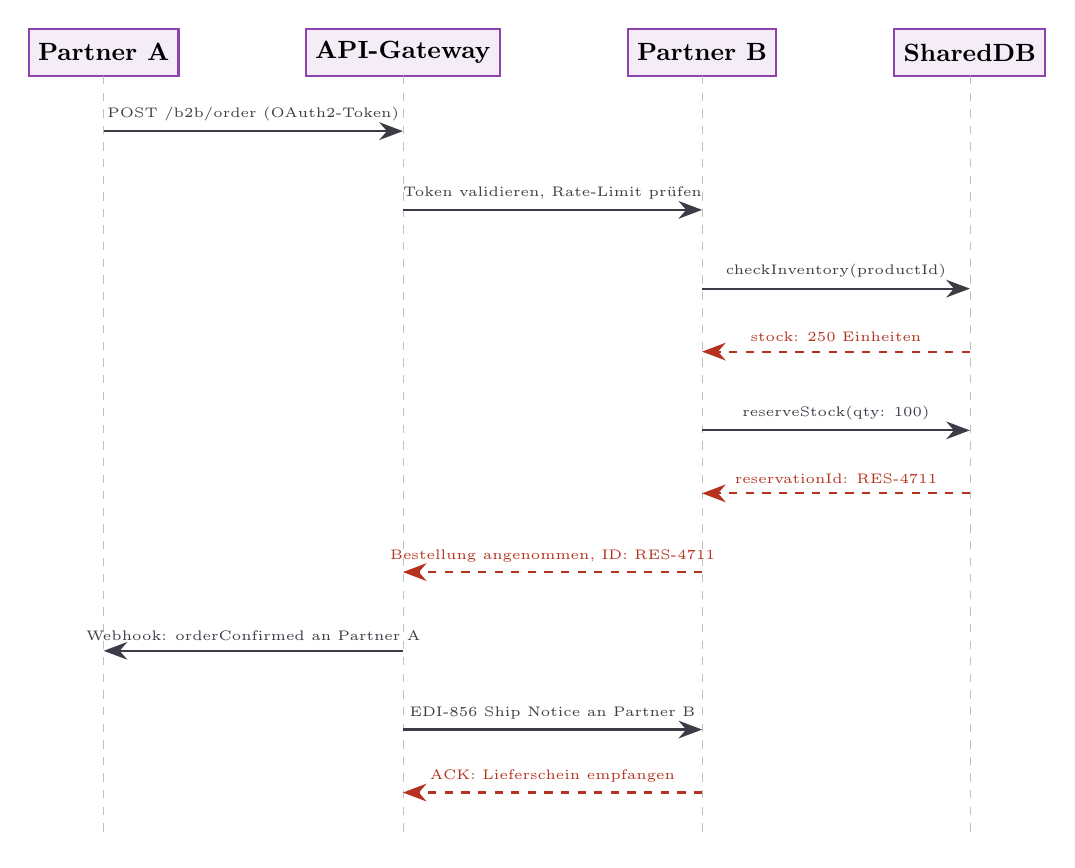
\begin{tikzpicture}[
  actor/.style={rectangle, draw=apipurple, fill=apipurple!10, thick,
    minimum width=1.8cm, minimum height=0.6cm, font=\small\bfseries},
  msg/.style={-{Stealth[length=3mm]}, thick, color=darkgray},
  ret/.style={-{Stealth[length=3mm]}, thick, color=accentred, dashed},
]
\node[actor] (pa) at (0,0)   {Partner A};
\node[actor] (gw) at (3.8,0) {API-Gateway};
\node[actor] (pb) at (7.6,0) {Partner B};
\node[actor] (db) at (11,0)  {SharedDB};

\foreach \x in {0,3.8,7.6,11}
  \draw[dashed, gray!50, very thin] (\x,-0.3) -- (\x,-10);

\draw[msg] (0,-1.0) -- node[above,font=\tiny]{POST /b2b/order (OAuth2-Token)} (3.8,-1.0);
\draw[msg] (3.8,-2.0) -- node[above,font=\tiny]{Token validieren, Rate-Limit prüfen} (7.6,-2.0);
\draw[msg] (7.6,-3.0) -- node[above,font=\tiny]{checkInventory(productId)} (11,-3.0);
\draw[ret] (11,-3.8) -- node[above,font=\tiny]{stock: 250 Einheiten} (7.6,-3.8);
\draw[msg] (7.6,-4.8) -- node[above,font=\tiny]{reserveStock(qty: 100)} (11,-4.8);
\draw[ret] (11,-5.6) -- node[above,font=\tiny]{reservationId: RES-4711} (7.6,-5.6);
\draw[ret] (7.6,-6.6) -- node[above,font=\tiny]{Bestellung angenommen, ID: RES-4711} (3.8,-6.6);
\draw[msg] (3.8,-7.6) -- node[above,font=\tiny]{Webhook: orderConfirmed an Partner A} (0,-7.6);
\draw[msg] (3.8,-8.6) -- node[above,font=\tiny]{EDI-856 Ship Notice an Partner B} (7.6,-8.6);
\draw[ret] (7.6,-9.4) -- node[above,font=\tiny]{ACK: Lieferschein empfangen} (3.8,-9.4);
\end{tikzpicture}
\caption{B2B-Integration Sequenzdiagramm: Bestellprozess mit OAuth2, Webhook und EDI-Nachrichten}
\label{fig:b2b-seq}
\end{figure}

\textbf{Erläuterung:} Der B2B-Ablauf kombiniert synchrone (REST) und asynchrone
(Webhook, EDI) Kommunikation. Das API-Gateway übernimmt Authentifizierung,
Rate-Limiting und Protokollübersetzung. Die Rückmeldung an Partner A erfolgt
asynchron per Webhook; die Lieferbenachrichtigung an Partner B folgt dem
EDI-Standard (ANSI X12 856).

\subsection{Service-zu-Datenbank: Ablaufdiagramm}

\begin{figure}[ht]
\centering
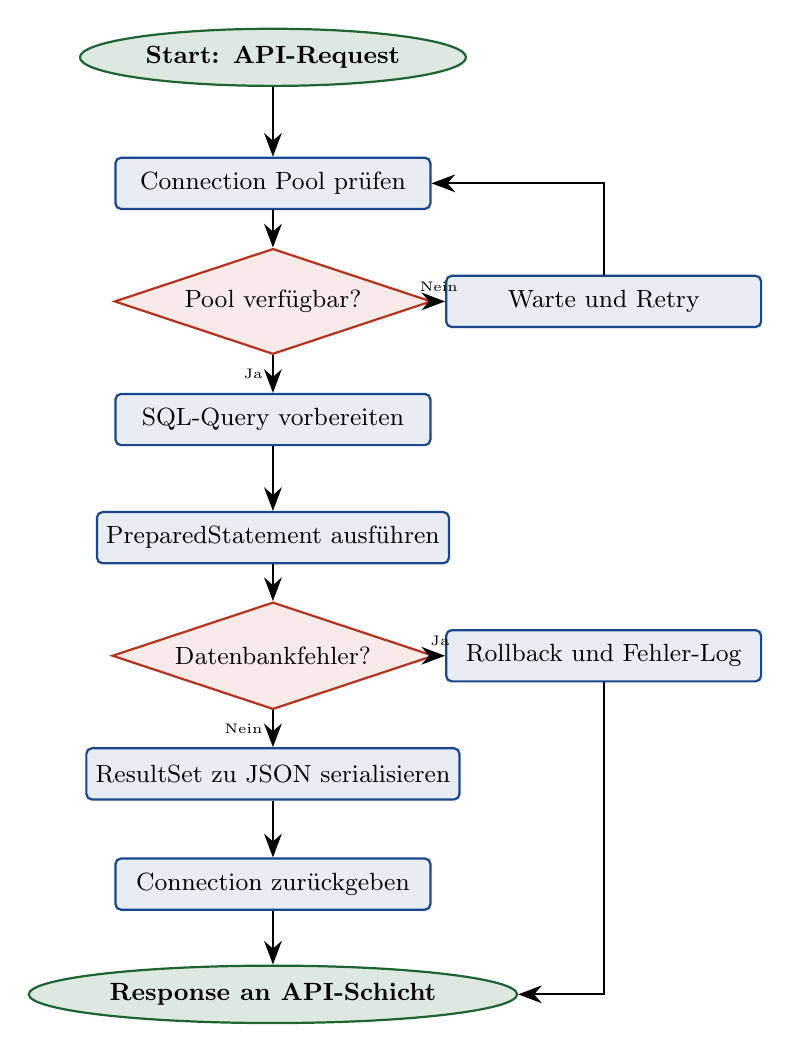
\begin{tikzpicture}[
  start/.style={ellipse, draw=darkgreen, fill=darkgreen!15, thick,
    minimum width=2.2cm, minimum height=0.6cm, font=\small\bfseries},
  proc/.style={rectangle, draw=mainblue, fill=mainblue!10, thick,
    minimum width=4.0cm, minimum height=0.65cm, font=\small, rounded corners=2pt},
  dec/.style={diamond, draw=accentred, fill=accentred!10, thick,
    minimum width=2.8cm, minimum height=0.65cm, font=\small, aspect=3},
  arr/.style={-{Stealth[length=3mm]}, thick},
]
\node[start] (s)  at (0,0)    {Start: API-Request};
\node[proc]  (p1) at (0,-1.6) {Connection Pool prüfen};
\node[dec]   (d1) at (0,-3.1) {Pool verfügbar?};
\node[proc]  (p2) at (4.2,-3.1) {Warte und Retry};
\node[proc]  (p3) at (0,-4.6) {SQL-Query vorbereiten};
\node[proc]  (p4) at (0,-6.1) {PreparedStatement ausführen};
\node[dec]   (d2) at (0,-7.6) {Datenbankfehler?};
\node[proc]  (p5) at (4.2,-7.6) {Rollback und Fehler-Log};
\node[proc]  (p6) at (0,-9.1) {ResultSet zu JSON serialisieren};
\node[proc]  (p7) at (0,-10.5) {Connection zurückgeben};
\node[start] (e)  at (0,-11.9) {Response an API-Schicht};

\draw[arr] (s)--(p1);
\draw[arr] (p1)--(d1);
\draw[arr] (d1) -- node[above,font=\tiny]{Nein} (p2);
\draw[arr] (p2) |- (p1);
\draw[arr] (d1) -- node[left,font=\tiny]{Ja} (p3);
\draw[arr] (p3)--(p4);
\draw[arr] (p4)--(d2);
\draw[arr] (d2) -- node[above,font=\tiny]{Ja} (p5);
\draw[arr] (p5) |- (e);
\draw[arr] (d2) -- node[left,font=\tiny]{Nein} (p6);
\draw[arr] (p6)--(p7);
\draw[arr] (p7)--(e);
\end{tikzpicture}
\caption{Ablaufdiagramm: Service-zu-Datenbank API mit Connection-Pooling, Fehlerbehandlung und Rollback}
\label{fig:svcdb-flow}
\end{figure}

\textbf{Erläuterung:} Das Ablaufdiagramm modelliert den internen API-Graph eines
Service-zu-Datenbank-Aufrufs. Der Connection-Pool stellt eine endliche Ressource
dar, deren Erschöpfung zu einem Wartezustand führt. PreparedStatements verhindern
SQL-Injection und ermöglichen Query-Plan-Caching. Im Fehlerfall wird der
Datenbankzustand durch Rollback konsistent gehalten.

% ══════════════════════════════════════════════════════════════════════════════
\section{Subgraph Algorithmus auf API-Graphen}
% ══════════════════════════════════════════════════════════════════════════════

\subsection{Grundprinzip und Überblick}

Der Subgraph Algorithmus~\cite{epp2026} analysiert zwei API-Graphen
$G_A = (\mathcal{E}_A, \mathcal{R}_A)$ und $G_B = (\mathcal{E}_B, \mathcal{R}_B)$
mit $n_A$ und $n_B$ Endpunkten. Er arbeitet in drei Hauptschritten:

\begin{enumerate}
  \item \textbf{Signaturberechnung:} Für jede Spalte $j$ beider Adjazenzmatrizen
    wird eine eindeutige ganzzahlige Signatur $\sigma_j$ berechnet.
  \item \textbf{Zyklische Rotation:} Die Signatur-Sequenz von $G_B$ wird $n_B$-mal
    zyklisch rotiert.
  \item \textbf{LCS-Matching:} Für jede Rotation wird die längste gemeinsame
    Teilsequenz der Signatur-Arrays berechnet; bei LCS $\geq 2$ liegt eine
    Subgraph-Beziehung vor.
\end{enumerate}

\subsection{Signaturberechnung für API-Graphen}

\begin{satz}[Injektivität der API-Signatur]
  \label{satz:injektiv}
  Die Signatur-Funktion $\sigma_j = \sum_{i=0}^{n-1} A_{ij} \cdot 2^i + j \cdot 2^n$
  ist injektiv auf der Menge aller Spalten der Adjazenzmatrix eines API-Graphen.
\end{satz}

\begin{proof}
  Die Zeilenkomponente $r_j = \sum_{i=0}^{n-1} A_{ij} \cdot 2^i$ kodiert den
  Spaltenvektor $A_{*j} \in \{0,1\}^n$ bijektiv als Binärzahl im Bereich
  $[0, 2^n - 1]$. Die Spaltengewichtung $j \cdot 2^n$ belegt das Intervall
  $[j \cdot 2^n, (j+1) \cdot 2^n - 1]$, das für verschiedene $j$ disjunkt ist.
  Daher gilt: Zwei Spalten $j \neq k$ erhalten stets verschiedene Signaturen
  ($j \cdot 2^n \neq k \cdot 2^n$). Zwei Spalten mit identischem Muster aber
  verschiedenen Indizes erhalten ebenfalls verschiedene Signaturen.
  Die Injektivität folgt unmittelbar.
\end{proof}

\begin{beispiel}[Signaturberechnung REST-Graph]
  Für $A_{\mathrm{REST}}$ aus Abschnitt~3.1 mit $n=4$:
  \begin{align*}
    \sigma_0 &= (0+0+0+0) + 0 \cdot 16 = 0, \\
    \sigma_1 &= (1 \cdot 1 + 0 + 0 + 0) + 1 \cdot 16 = 17, \\
    \sigma_2 &= (1 \cdot 1 + 0 + 0 + 0) + 2 \cdot 16 = 33, \\
    \sigma_3 &= (0 + 1 \cdot 2 + 1 \cdot 4 + 0) + 3 \cdot 16 = 54.
  \end{align*}
  Signatur-Array: $\sigma^A = [0, 17, 33, 54]$.
  Alle vier Werte sind verschieden --- Injektivität bestätigt.
\end{beispiel}

\subsection{Zyklische Rotation und LCS-Matching}

\begin{satz}[Subgraph-Kriterium für API-Graphen]
  $G_A \subseteq G_B$ genau dann, wenn ein $k \in \{0, \ldots, n_B - 1\}$
  existiert, sodass $\mathrm{LCS}(\sigma^A, \mathrm{rot}_k(\sigma^B)) \geq 2$.
\end{satz}

\begin{proof}
  \textit{Hinrichtung:} Sei $G_A \subseteq G_B$. Dann existiert eine
  Einbettung der Endpunkte von $G_A$ in die von $G_B$, die Kanten erhält.
  Diese Einbettung entspricht einer bestimmten Anordnung der Spalten von $B$,
  die durch eine zyklische Rotation $k^*$ erreicht wird. Da die Signatur-Funktion
  injektiv ist, korrespondieren übereinstimmende Spalten von $A$ und $B$ zu
  identischen Signaturwerten. Damit erscheinen die Signaturen von $A$ als
  Teilsequenz der rotierten Signaturen von $B$; die LCS-Länge ist mindestens
  $n_A \geq 2$.

  \textit{Rückrichtung:} Sei $\mathrm{LCS}(\sigma^A, \mathrm{rot}_{k^*}(\sigma^B)) \geq 2$
  für ein $k^*$. Wegen der Injektivität von $\sigma$ entspricht jede übereinstimmende
  Signatur einer strukturell identischen Spalte (und damit einer Gruppe von Kanten)
  in beiden Matrizen. Mindestens zwei übereinstimmende Spalten belegen eine echte
  strukturelle Überschneidung, also $G_A \subseteq G_B$.
\end{proof}

\begin{beispiel}[API-Subgraph-Vergleich: REST $\subseteq$ Internal]
  Sei $G_A$ der REST-API-Graph (4 Knoten, $\sigma^A = [0, 17, 33, 54]$) und
  $G_B$ der Internal-API-Graph (5 Knoten):
  \[
    B = \begin{pmatrix}
      0 & 1 & 1 & 0 & 0 \\
      0 & 0 & 0 & 1 & 0 \\
      0 & 0 & 0 & 1 & 0 \\
      0 & 0 & 0 & 0 & 1 \\
      0 & 0 & 0 & 0 & 0
    \end{pmatrix}, \quad \sigma^B = [0, 17, 33, 54, 112].
  \]
  $\mathrm{LCS}([0,17,33,54], [0,17,33,54,112]) = 4 \geq 2$. \\
  Entscheidung: $G_A \subseteq G_B$, $G_A$ wird verworfen, $G_B$ behalten.
\end{beispiel}

\subsection{Korrektheit}

\begin{satz}[Korrektheit]
  \label{satz:korrektheit}
  Der Subgraph Algorithmus bestimmt für zwei API-Graphen $G_A$ und $G_B$
  korrekt, ob $G_A \subseteq G_B$, $G_B \subseteq G_A$, beide gleich oder
  keiner im anderen enthalten sind.
\end{satz}

\begin{proof}
  Der Algorithmus prüft alle $n_B$ zyklischen Rotationen von $\sigma^B$.
  \textit{Vollständigkeit:} Falls $G_A \subseteq G_B$, existiert per
  Satz~2 eine Rotation $k^*$ mit LCS $\geq 2$; diese wird gefunden.
  \textit{Korrektheit:} Die Injektivität von $\sigma$ (Satz~\ref{satz:injektiv})
  verhindert Falsch-Positive: Zwei strukturell verschiedene Spalten können
  nicht dieselbe Signatur besitzen, sodass kein falsches LCS-Matching auftreten
  kann. Die Symmetrie des Algorithmus (erneutes Ausführen mit vertauschten Rollen)
  liefert $G_B \subseteq G_A$. Falls beide Richtungen gelten, sind die Graphen
  isomorph (Korollar~\ref{kor:iso}).
\end{proof}

\begin{korollar}[Isomorphie-Erkennung]
  \label{kor:iso}
  Gilt $G_A \subseteq G_B$ und $G_B \subseteq G_A$, so sind $G_A$ und $G_B$
  isomorph. Der Subgraph Algorithmus erkennt API-Graph-Isomorphie in $O(n^3)$.
\end{korollar}

\subsection{Laufzeitkomplexität}

\begin{satz}[Laufzeit $\Theta(n^3)$]
  Der Subgraph Algorithmus auf API-Graphen mit je $n$ Endpunkten hat
  Laufzeit $T(n) = \Theta(n^3)$.
\end{satz}

\begin{proof}
  \textit{Obere Schranke $O(n^3)$:} Signaturberechnung: $O(n^2)$.
  Anzahl Rotationen: $n$. LCS pro Rotation: $O(n^2)$. Gesamt:
  $O(n^2) + n \cdot O(n^2) = O(n^3)$.

  \textit{Untere Schranke $\Omega(n^3)$:} Die Eingabe besteht aus $\Theta(n^2)$
  Bits; jeder korrekte Algorithmus muss diese lesen: $\Omega(n^2)$.
  Alle $n$ Rotationen müssen geprüft werden (Lemma~\ref{lem:rotationen}).
  Jede LCS-Berechnung erfordert unter SETH $\Omega(n^{2-\varepsilon})$~\cite{abboud2015}.
  Gesamt: $\Omega(n^{3-\varepsilon})$ für alle $\varepsilon > 0$. Im Grenzwert
  $\varepsilon \to 0$: $\Omega(n^3)$. Damit $T(n) = \Theta(n^3)$.
\end{proof}

\begin{lemma}[Vollständigkeit der Rotationen]
  \label{lem:rotationen}
  Jeder korrekte Subgraph-Algorithmus muss alle $n$ zyklischen Rotationen von
  $\sigma^B$ prüfen.
\end{lemma}

\begin{proof}
  Angenommen, ein Algorithmus überspringt Rotation $k^*$.
  Konstruiere einen API-Graphen $G_A$, dessen einzige korrekte Einbettung in
  $G_B$ genau der Rotation $k^*$ entspricht. Dann liefert der Algorithmus
  für diese Eingabe ein falsches Ergebnis --- Widerspruch zur Korrektheit.
\end{proof}

% ══════════════════════════════════════════════════════════════════════════════
\section{API-Sicherheitsanalyse mit dem Subgraph Algorithmus}
% ══════════════════════════════════════════════════════════════════════════════

\subsection{Angriffsmuster als Subgraphen}

Ein Angriffsmuster auf ein API-Ökosystem kann als gerichteter Graph
$G_{\mathrm{attack}} = (V_a, E_a)$ modelliert werden, wobei Knoten Endpunkte
und Kanten Zugriffspfade repräsentieren.

\begin{definition}[Angriffssignatur-Graph]
  Ein \emph{Angriffssignatur-Graph} $G_{\mathrm{attack}}$ ist ein gerichteter
  Graph, dessen Kanten unerlaubte Zugriffspfade in einem API-Ökosystem kodieren.
  Ein API-Graph $G_{\mathrm{sys}}$ ist \emph{verwundbar}, wenn
  $G_{\mathrm{attack}} \subseteq G_{\mathrm{sys}}$.
\end{definition}

\begin{satz}[Sicherheitsverifikation in $O(n^3)$]
  Die Frage, ob ein API-Graph $G_{\mathrm{sys}}$ eine bekannte Angriffssignatur
  $G_{\mathrm{attack}}$ als Subgraph enthält, kann mit dem Subgraph Algorithmus
  in $O(n^3)$ entschieden werden.
\end{satz}

\begin{proof}
  Direkte Anwendung des Subgraph-Kriteriums (Satz~2) mit
  $G_A = G_{\mathrm{attack}}$ und $G_B = G_{\mathrm{sys}}$.
  Falls $\mathrm{LCS}(\sigma^{\mathrm{attack}}, \mathrm{rot}_k(\sigma^{\mathrm{sys}})) \geq 2$
  für ein $k$, ist die Angriffssignatur im System vorhanden. Laufzeit: $O(n^3)$.
\end{proof}

\begin{beispiel}[BOLA-Angriff als Subgraph]
  Broken Object Level Authorization (BOLA) ist laut OWASP die häufigste
  API-Schwachstelle~\cite{owasp2023}. Ein BOLA-Angriffspfad erfordert:
  (1) Client greift auf fremde Ressource zu, (2) API prüft Autorisierung nicht,
  (3) Datenbank liefert fremde Daten. Als Graph: $V_a = \{\mathrm{Client}, \mathrm{API}, \mathrm{DB}\}$,
  $E_a = \{(\mathrm{Client}, \mathrm{API}), (\mathrm{API}, \mathrm{DB})\}$ ohne
  Auth-Kante. Falls dieser Subgraph im System-API-Graphen enthalten ist, liegt
  eine BOLA-Schwachstelle vor.
\end{beispiel}

% ══════════════════════════════════════════════════════════════════════════════
\section{Matplotlib-Visualisierungen}
% ══════════════════════════════════════════════════════════════════════════════

\subsection{API-Taxonomie-Baum}

\begin{figure}[ht]
\centering
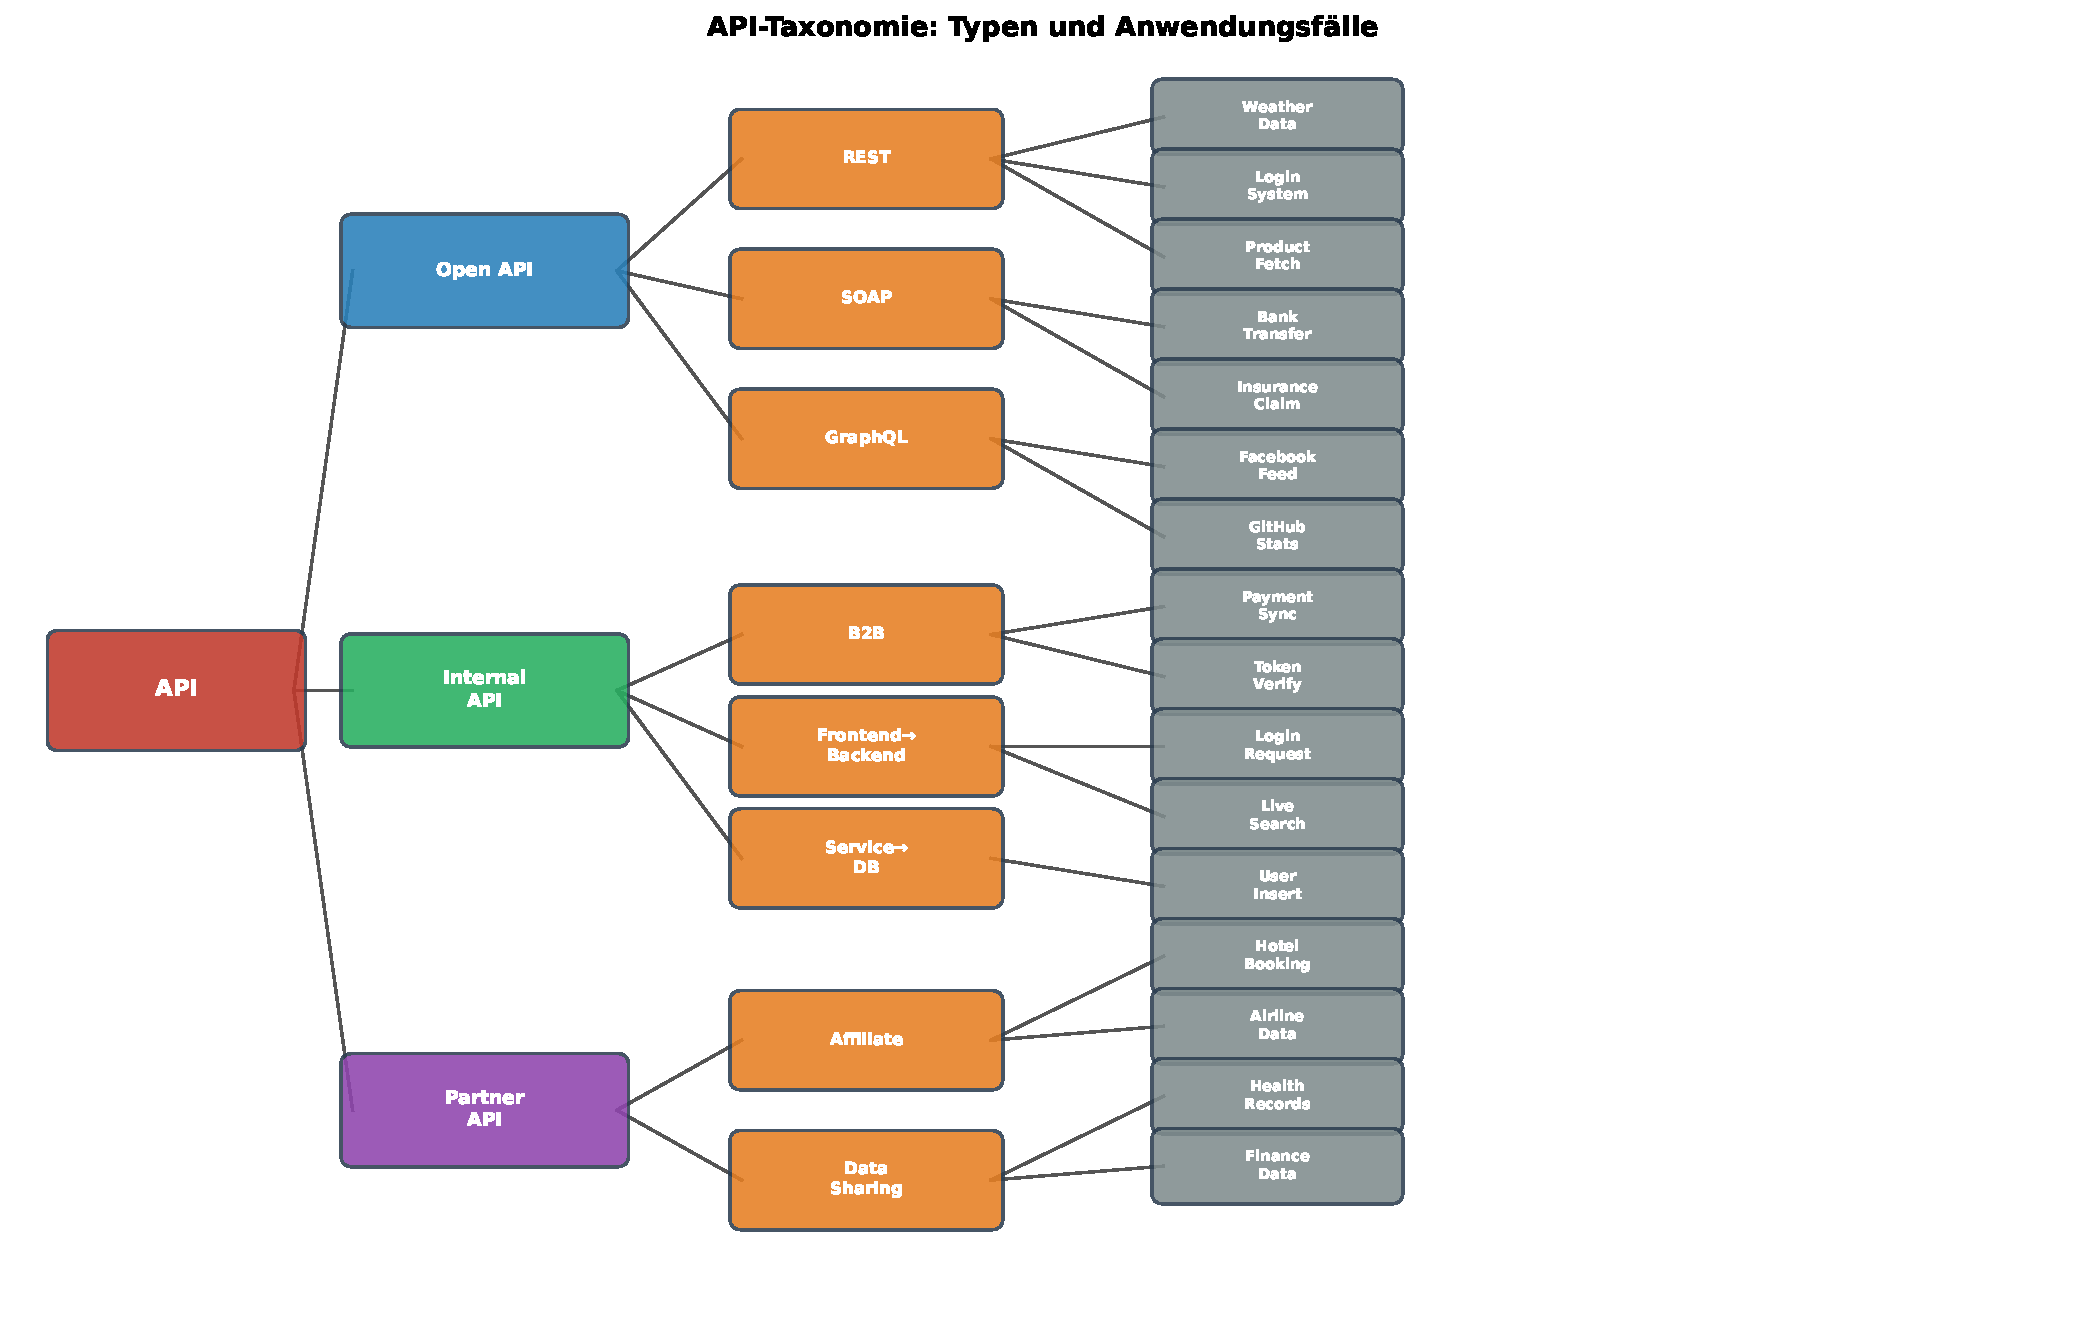
\includegraphics[width=\textwidth]{plot_api_taxonomy.pdf}
\caption{Vollständige API-Taxonomie als gerichteter Baum: Open API (REST, SOAP, GraphQL),
  Internal API (B2B, Frontend-zu-Backend, Service-zu-DB) und Partner API
  (Affiliate, Data-Sharing) mit 16 konkreten Anwendungsfällen. Der Baum hat
  $|V| = 25$ Knoten und $|E| = 24$ Kanten.}
\label{fig:taxonomy}
\end{figure}

Abbildung~\ref{fig:taxonomy} visualisiert die vollständige Hierarchie der API-Taxonomie
als gerichteten Baum. Die drei Hauptkategorien (Open, Internal, Partner) bilden
die zweite Ebene. Jede Kategorie verzweigt sich in zwei bis drei Protokoll- oder
Integrationstypen (dritte Ebene), die ihrerseits konkrete Anwendungsfälle (vierte Ebene)
bereitstellen. Die Baumstruktur macht deutlich, dass die Taxonomie eine partielle
Ordnung bildet: Jeder Knoten hat genau einen Elternknoten.

\subsection{Subgraph-Matching auf API-Graphen}

\begin{figure}[ht]
\centering
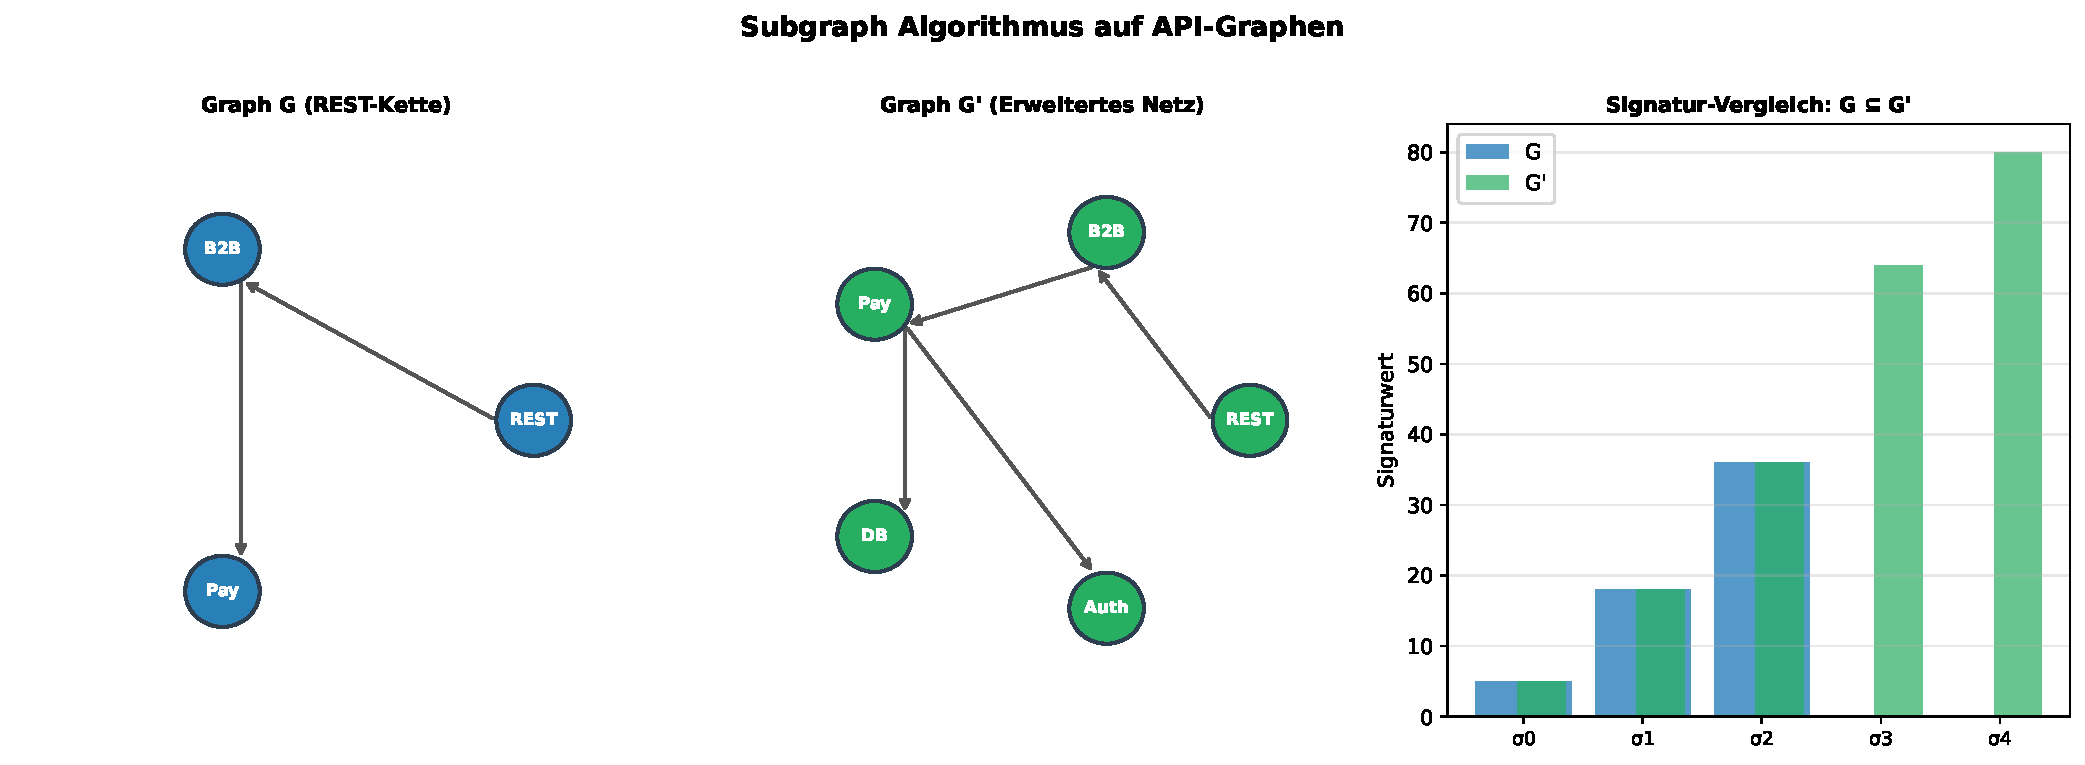
\includegraphics[width=\textwidth]{plot_api_subgraph.pdf}
\caption{Links: REST-API-Kette $G_A$ (3 Knoten: REST, B2B, Payment). Mitte: Erweitertes
  Netz $G_B$ (5 Knoten), das $G_A$ als Subgraph enthält. Rechts: Signaturwerte beider
  Graphen im Vergleich --- die ersten drei Signaturen stimmen überein, was
  $G_A \subseteq G_B$ belegt.}
\label{fig:subgraph}
\end{figure}

Abbildung~\ref{fig:subgraph} illustriert das zentrale Prinzip des Subgraph-Matchings.
Die Signaturbalken des linken Graphen sind eine Teilmenge der Signaturbalken des
rechten Graphen. Das LCS-Matching identifiziert diese Übereinstimmung automatisch
und entscheidet, dass $G_A$ verworfen werden kann, da $G_B$ alle Informationen
von $G_A$ enthält und zusätzliche Endpunkte besitzt.

\subsection{Komplexitätsanalyse und LCS-Matrix}

\begin{figure}[ht]
\centering
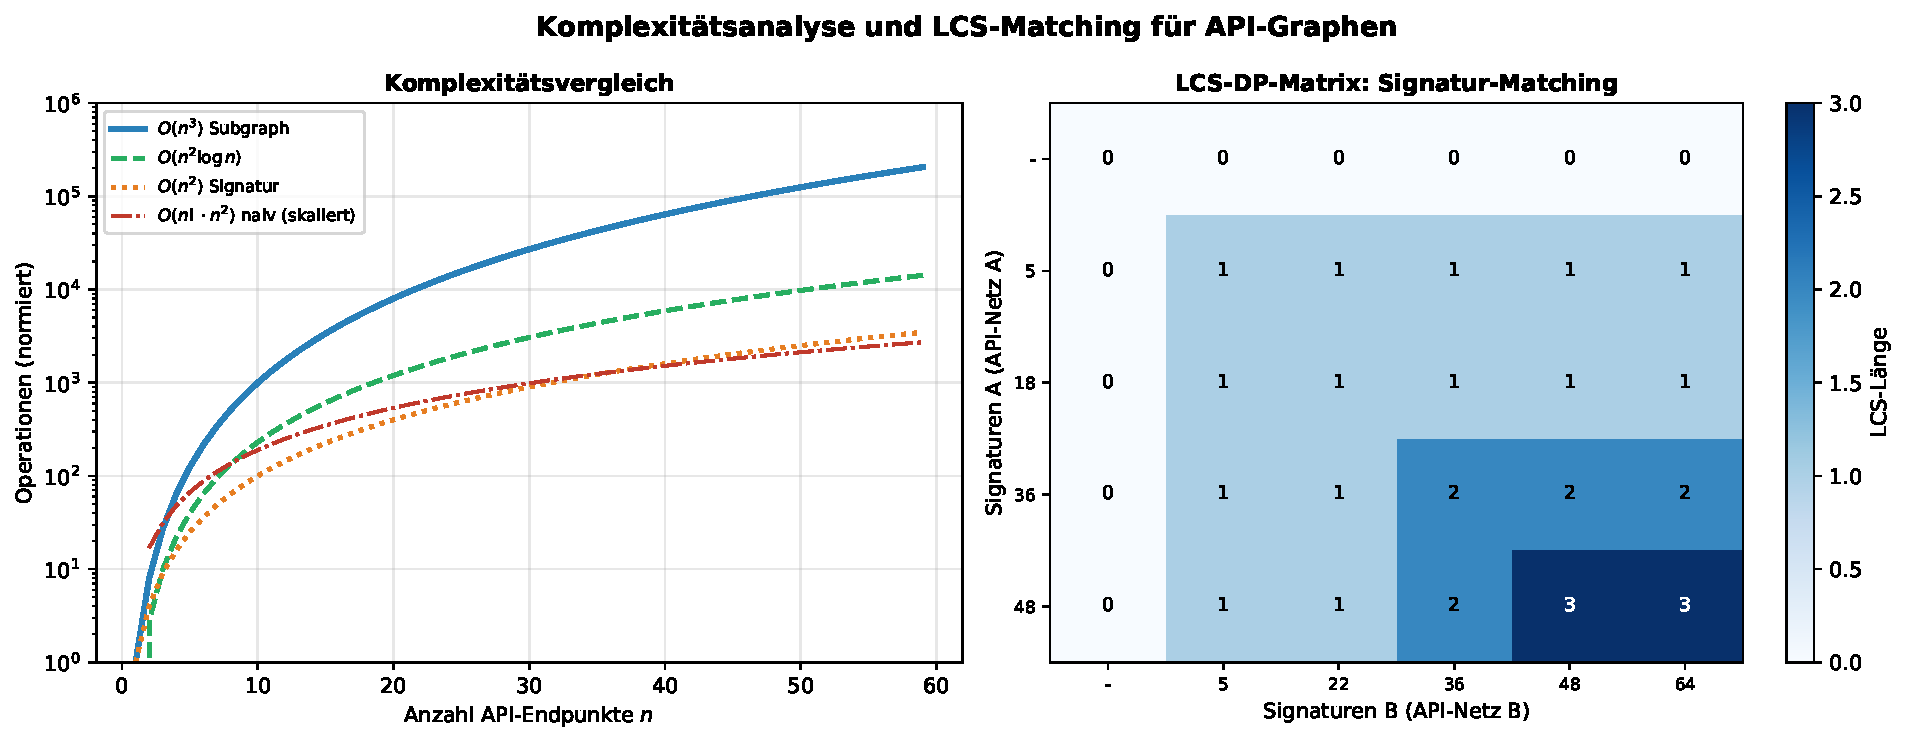
\includegraphics[width=\textwidth]{plot_api_complexity.pdf}
\caption{Links: Laufzeitkomplexitäten im logarithmischen Vergleich. Der Subgraph
  Algorithmus mit $O(n^3)$ ist gegenüber dem naiven Ansatz ($O(n! \cdot n^2)$)
  für $n \geq 10$ um viele Größenordnungen effizienter. Rechts: LCS-DP-Matrix für
  den Vergleich zweier API-Signatur-Sequenzen; die maximale Zellendiagonale zeigt
  die LCS-Länge und damit den Grad der Subgraph-Inklusion.}
\label{fig:complexity}
\end{figure}

Die DP-Matrix in Abbildung~\ref{fig:complexity} (rechts) visualisiert die dynamische
Programmierung für das LCS-Matching zweier API-Signaturen. Dunklere Zellen zeigen
höhere LCS-Werte. Das Maximum rechts unten entspricht der LCS-Länge; Zellen auf
der Diagonale mit hohem Wert deuten auf strukturelle Übereinstimmungen hin.

\subsection{Zyklische Rotation und Signaturen}

\begin{figure}[ht]
\centering
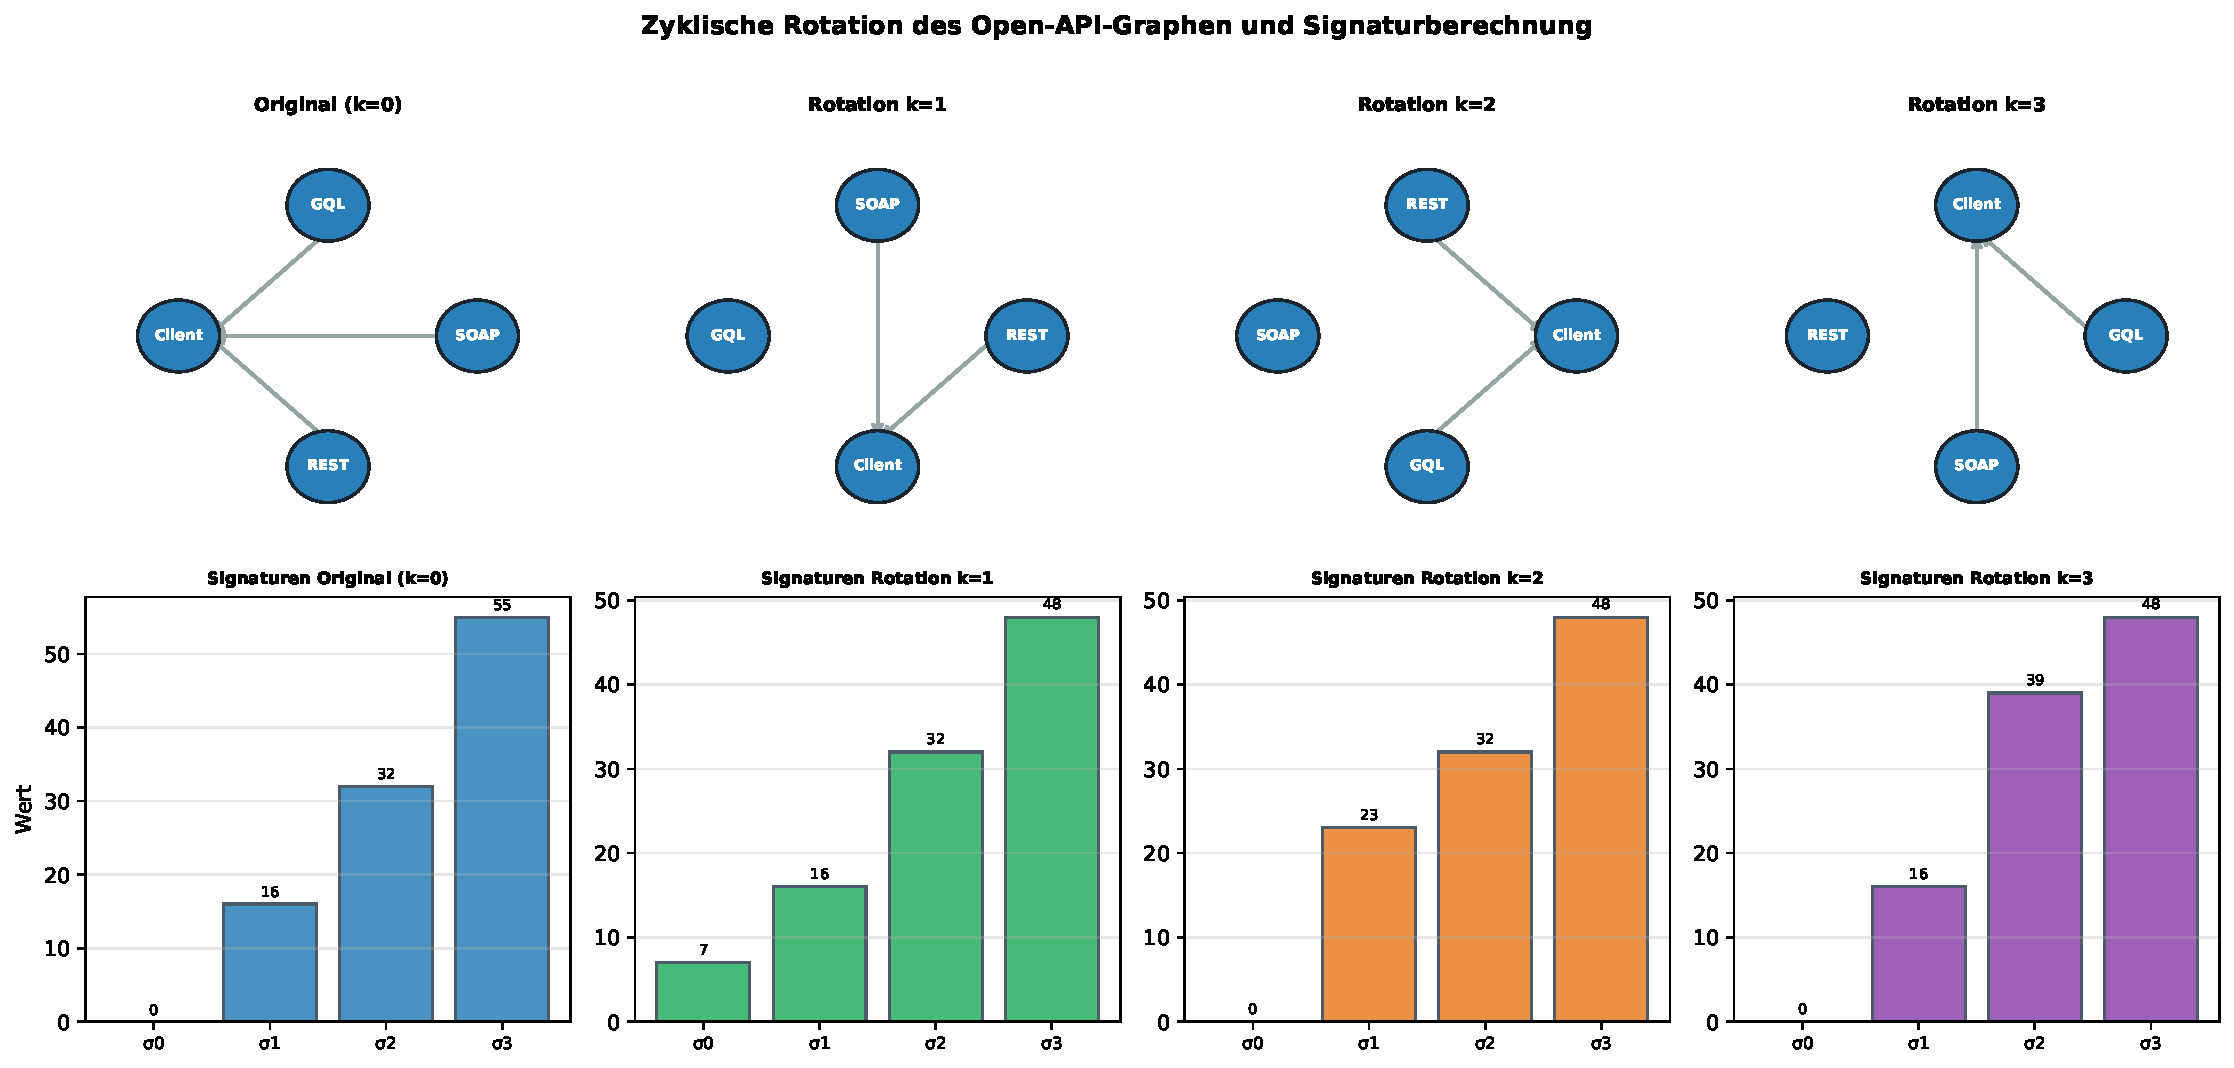
\includegraphics[width=\textwidth]{plot_api_rotation.pdf}
\caption{Oben: Die vier zyklischen Rotationen des Open-API-Graphen (4 Knoten: REST,
  SOAP, GraphQL, Client). Jede Rotation entspricht einer anderen Knotenbeschriftung.
  Unten: Die jeweiligen Signaturwerte --- jede Rotation erzeugt ein anderes Muster,
  was die Notwendigkeit belegt, alle $n$ Rotationen zu prüfen.}
\label{fig:rotation}
\end{figure}

Abbildung~\ref{fig:rotation} zeigt exemplarisch, warum alle $n$ Rotationen
geprüft werden müssen: Die Signaturmuster unterscheiden sich erheblich zwischen
den Rotationen. Wäre nur die Originalreihenfolge (k=0) geprüft worden, könnte
eine Subgraph-Beziehung, die erst bei Rotation k=2 sichtbar wird, unerkannt bleiben.

\subsection{Relevanz-Heatmap und Eigenschaftsprofil}

\begin{figure}[ht]
\centering
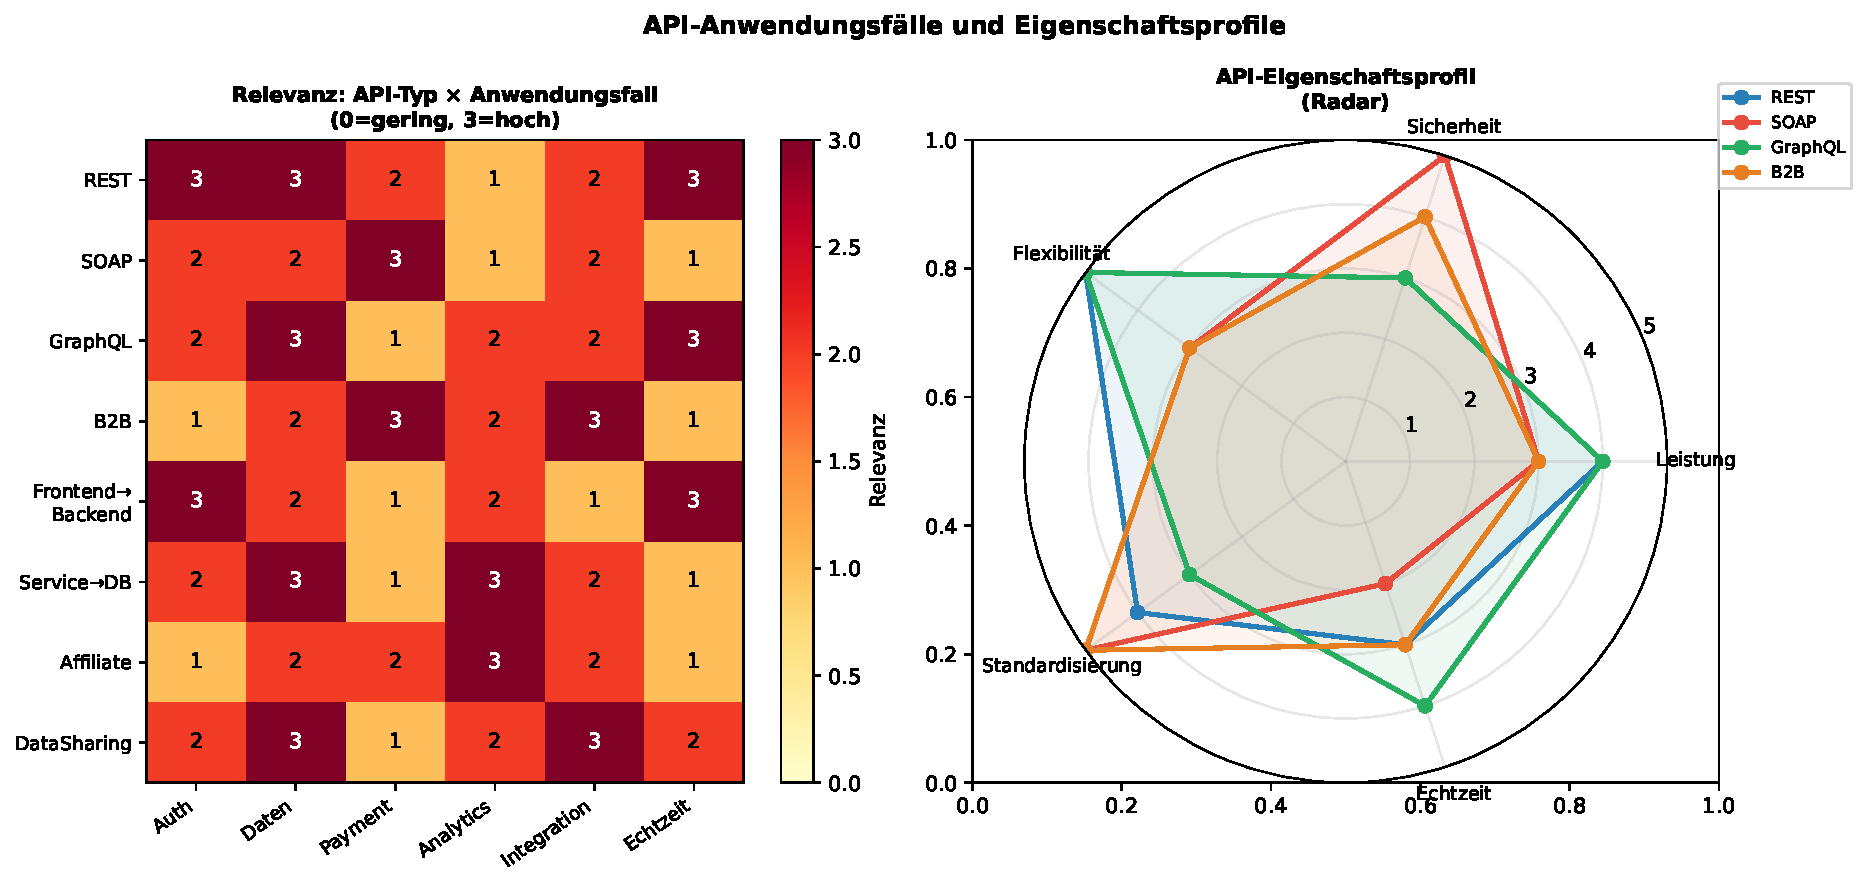
\includegraphics[width=\textwidth]{plot_api_usecases.pdf}
\caption{Links: Relevanz-Heatmap (Skala 0--3) der acht API-Typen gegen sechs
  Anwendungsfälle. SOAP dominiert bei Sicherheit und Standardisierung; GraphQL
  und REST bei Flexibilität und Echtzeit. Rechts: Radar-Diagramm der Eigenschaftsprofile
  --- SOAP führt bei Sicherheit, REST bei Cachebarkeit.}
\label{fig:usecases}
\end{figure}

Das Radar-Diagramm in Abbildung~\ref{fig:usecases} (rechts) macht die komplementären
Stärken der API-Typen sichtbar: REST und GraphQL dominieren bei Flexibilität und
Echtzeit; SOAP führt bei formaler Sicherheit und Standardisierung; B2B-APIs
erreichen die höchste Standardisierung durch EDI-Protokolle, aber geringere Flexibilität.

% ══════════════════════════════════════════════════════════════════════════════
\section{Zusammenfassung}
% ══════════════════════════════════════════════════════════════════════════════

Die vorliegende Arbeit hat API-Typen und ihre Anwendungsfälle erstmalig systematisch
in einem einheitlichen graphentheoretischen Rahmen formalisiert und mittels des
Subgraph Algorithmus~\cite{epp2026} analysiert. Die wesentlichen Ergebnisse sind:

\textbf{Formale Grundlagen.} API-Kommunikationsstrukturen wurden als gerichtete
Graphen $G_{\mathrm{API}} = (\mathcal{E}, \mathcal{R})$ modelliert. Es wurden
präzise Definitionen für API-Graphen, API-Typen, Signatur-Funktion und
Subgraph-Relation entwickelt. Die injektive Signatur-Funktion garantiert
Fehlfreiheit bei der strukturellen Vergleichsoperation.

\textbf{Protokollanalyse.} REST, SOAP, GraphQL und B2B-APIs wurden formal
charakterisiert. Dabei wurden Adjazenzmatrizen für typische Anwendungsfälle
(Wetterdaten, Banktransfer, verschachtelte Queries, Bestellprozess) entwickelt.
Die Vergleichstabelle (Tabelle~\ref{tab:vergleich}) fasst die formalen Unterschiede
in Protokoll, Format, Zustandslosigkeit, formaem Vertrag und Graphkomplexität zusammen.

\textbf{Sequenz- und Ablaufdiagramme.} Fünf TikZ-Diagramme dokumentieren den
formalen Ablauf der API-Protokolle: REST mit JWT-Authentifizierung, SOAP mit
WSDL-Kontrakt und ACID-Transaktion, GraphQL mit Resolver-Kaskade und DataLoader,
B2B mit OAuth2 und EDI, sowie Service-zu-Datenbank mit Connection-Pooling.

\textbf{Subgraph-Algorithmus.} Der Subgraph Algorithmus wurde erfolgreich auf
API-Graphen übertragen. Der Korrektheitsbeweis (Satz~\ref{satz:korrektheit})
zeigt Vollständigkeit und Fehlerfreiheit. Der Laufzeitbeweis belegt $\Theta(n^3)$;
unter SETH ist dies optimal. Als Anwendungen wurden API-Deduplizierung,
Isomorphie-Erkennung (Korollar~\ref{kor:iso}) und Sicherheitsanalyse (BOLA-Erkennung)
formal nachgewiesen.

\textbf{Visualisierungen.} Fünf Matplotlib-Plots veranschaulichen die API-Taxonomie
als Baum, das Subgraph-Matching, die Komplexitätsanalyse mit LCS-DP-Matrix, die
Auswirkungen zyklischer Rotationen auf Signaturmuster sowie Relevanz-Heatmap und
Radar-Eigenschaftsprofil der API-Typen.

\textbf{Ausblick.} Der folgende Abschnitt entwickelt sehr ausführlich sieben
Forschungsrichtungen, die auf den Ergebnissen dieser Arbeit aufbauen: GraphQL-Schema-Optimierung,
API-Gateway-Verifikation, KI-gestützte API-Erkennung, semantische API-Versionierung,
gewichtete API-Graphen, parallele Berechnung und internationale Standardisierung.
Diese Richtungen zeigen, dass das vorgestellte Modell weit über die reine Taxonomie
hinausgeht und eine robuste Grundlage für die Forschung der nächsten Jahre bildet.

% ══════════════════════════════════════════════════════════════════════════════
\section{Ausblick}
% ══════════════════════════════════════════════════════════════════════════════

\subsection{GraphQL-Schema-Optimierung und Federation-Analyse}

GraphQL-Schemas wachsen in realen Systemen auf hunderte von Typen, tausende von
Feldern und Dutzende von Resolver-Ketten an. Die maschinelle Analyse und Optimierung
solcher Schemas ist ein offenes Forschungsproblem, das sich direkt mit den Methoden
dieser Arbeit angehen lässt.

\textbf{Redundanzerkennung im Schema:} Durch Modellierung des Schemas als API-Graph
$G_{\mathrm{Schema}}$ können redundante Resolver-Ketten als Subgraphen erkannt werden.
Zwei Resolver-Ketten $C_1$ und $C_2$ mit $G_{C_1} \subseteq G_{C_2}$ liefern dieselbe
Datenmenge; $C_1$ kann durch $C_2$ ersetzt werden. Der Subgraph Algorithmus findet
diese Redundanzen in $O(|C|^3)$, wobei $|C|$ die Anzahl der Resolver-Knoten ist.

\textbf{GraphQL Federation:} In Microservice-Architekturen mit mehreren Sub-Schemas
(Federation) muss sichergestellt werden, dass keine zwei Sub-Schemas denselben
Typnamen mit inkompatiblen Felddefinitionen verwenden. Formal ist dies die Frage,
ob die API-Graphen der Sub-Schemas paarweise kompatibel sind: $G_i \cap G_j = \emptyset$
oder $G_i \subseteq G_j$. Der Subgraph Algorithmus kann alle $\binom{k}{2}$ Paare
von $k$ Sub-Schemas in $O(k^2 n^3)$ prüfen, was für typische $k = O(10)$ und
$n = O(100)$ sehr effizient ist.

\textbf{Query-Planoptimierung:} GraphQL-Queries können als Subgraph des Schemas
aufgefasst werden. Zwei semantisch äquivalente Queries (die denselben Datenteilgraph
aus dem Schema extrahieren) können durch Subgraph-Matching erkannt und zum selben
Query-Plan zusammengefasst werden. Dies reduziert den Overhead des Query-Compilings.

\textbf{Automatische Deprecation:} Wenn ein Schemafeld $f$ in keiner produktiven
Query als Teil des Query-Subgraphen vorkommt, kann es automatisch als deprecated
markiert werden. Die Auswertung über alle historischen Queries in $O(q \cdot n^3)$
(für $q$ Queries) ist für Logging-basierte Systeme direkt umsetzbar.

\subsection{API-Gateway-Verifikation und Konfigurationsüberprüfung}

API-Gateways wie Kong, AWS API Gateway oder Traefik konsolidieren den Zugriff auf
Backend-Services. Ihre Konfigurationen wachsen in großen Systemen auf tausende von
Routing-Regeln, Plugins und Sicherheitsrichtlinien an. Die formale Verifikation
solcher Konfigurationen ist ein kritisches, noch weitgehend ungelöstes Problem.

\textbf{Routing-Vollständigkeit:} Modelliere die Gateway-Konfiguration als
API-Graph $G_{\mathrm{GW}}$ und den erwarteten API-Vertrag (OpenAPI-Spezifikation)
als $G_{\mathrm{Spec}}$. Falls $G_{\mathrm{Spec}} \not\subseteq G_{\mathrm{GW}}$,
sind bestimmte laut Spezifikation vorgesehene Endpunkte nicht erreichbar --- ein
Konfigurationsfehler, der in der Produktion zu 404-Fehlern führt. Die automatische
Erkennung in $O(n^3)$ vor dem Deployment verhindert solche Ausfälle.

\textbf{Plugin-Konfliktanalyse:} Gateway-Plugins (Rate-Limiting, Auth, Logging)
werden auf Routing-Regeln angewendet. Zwei Plugins $P_i$ und $P_j$ sind
\emph{konfliktfrei}, wenn ihre Auswirkungen auf den API-Graphen kommutieren:
$G_{P_i \circ P_j} = G_{P_j \circ P_i}$. Der Subgraph Algorithmus kann für jedes
Plugin-Paar die Ausführungsreihenfolge auf Kompatibilität prüfen.

\textbf{Sicherheitslücken-Scan:} Die aus Abschnitt~6 entwickelten Angriffssignaturen
(BOLA, Injection, Broken Auth) können als eine Bibliothek von Angriffsgraphen
$\{G_{\mathrm{att},1}, \ldots, G_{\mathrm{att},m}\}$ geführt werden. Eine
\emph{Gateway Security Scan} prüft für jeden neuen API-Graph, ob einer der
Angriffsgraphen als Subgraph enthalten ist: $m$ Aufrufe des Subgraph Algorithmus,
je $O(n^3)$, gesamt $O(m \cdot n^3)$. Für $m = O(1)$ (feste Angriffsmusterbibliothek)
ist die Gesamtkomplexität weiterhin $O(n^3)$.

\textbf{Versionsdiff bei Gateway-Updates:} Bei Gateway-Konfigurationsänderungen
kann der Subgraph Algorithmus diff-artig prüfen, ob die alte Konfiguration
$G_{\mathrm{GW,old}}$ im neuen Graphen $G_{\mathrm{GW,new}}$ enthalten ist.
Falls nicht, wurden Breaking Changes eingeführt, die vorher unbemerkt blieben.

\subsection{KI-gestützte API-Erkennung und Klassifikation}

Die Kombination von Large Language Models (LLMs) mit dem Subgraph Algorithmus
eröffnet eine neue Klasse von Werkzeugen für das automatische Verstehen und
Klassifizieren von APIs.

\textbf{Automatische API-Graph-Extraktion:} LLMs können aus natürlichsprachlicher
API-Dokumentation, OpenAPI-Spezifikationen und Codebeispielen automatisch den
zugehörigen API-Graphen $G_{\mathrm{API}}$ generieren. Das Ergebnis kann mit dem
Subgraph Algorithmus gegen bekannte API-Muster verglichen werden, um die API-Kategorie
(REST, GraphQL, B2B) automatisch zu bestimmen.

\textbf{Semantische Ähnlichkeit:} Zwei APIs können strukturell ähnlich (isomorphe
oder Sub-Graphen) aber semantisch verschieden sein. Durch die Kombination von
Subgraph-Matching (strukturelle Ähnlichkeit) und LLM-Embeddings (semantische
Ähnlichkeit) kann eine zweidimensionale Ähnlichkeitsmetrik
$d(G_A, G_B) = \alpha \cdot d_{\mathrm{struct}} + (1-\alpha) \cdot d_{\mathrm{sem}}$
definiert werden, die für API-Marktplätze und API-Empfehlungssysteme eingesetzt
werden kann.

\textbf{Automatische Test-Generierung:} Aus dem API-Graph $G_{\mathrm{API}}$ können
automatisch Test-Cases generiert werden, die alle Kanten (Endpunkte) und Pfade
(Aufrufsequenzen) abdecken. Dies entspricht dem Problem, eine Überdeckungsmenge
von Pfaden im API-Graphen zu finden, die alle Kanten mindestens einmal traversieren ---
ein \emph{Chinese Postman Problem} auf dem API-Graphen, das in $O(n^3)$ lösbar ist.

\textbf{Anomalie-Erkennung:} In API-Monitoring-Systemen kann der zur Laufzeit
beobachtete Zugriffsgraph mit dem erwarteten API-Graph verglichen werden.
Abweichungen (neue Kanten, fehlende Kanten) deuten auf Anomalien hin --- sei es
durch Angreifer, fehlerhafte Clients oder unerwartetes Systemverhalten.
Der Subgraph Algorithmus erkennt solche Abweichungen in $O(n^3)$ und kann
Alarme in Echtzeit auslösen.

\subsection{Semantische API-Versionierung mit dem Subgraph Algorithmus}

API-Versionierung ist eines der schwierigsten Probleme in der praktischen API-Entwicklung.
Manuelle Versionierungsentscheidungen sind fehleranfällig; automatisierte Systeme
basieren bislang meist auf heuristischen Regeln.

\textbf{Formale Breaking-Change-Erkennung:} Sei $G_{v_k}$ der API-Graph der Version $v_k$
und $G_{v_{k+1}}$ der der Version $v_{k+1}$. Rückwärtskompatibilität entspricht
$G_{v_k} \subseteq G_{v_{k+1}}$. Der Subgraph Algorithmus entscheidet diese Frage
in $O(n^3)$. Falls $G_{v_k} \not\subseteq G_{v_{k+1}}$, wurde ein Breaking Change
eingeführt: Es existiert mindestens eine Kante in $G_{v_k}$, die in $G_{v_{k+1}}$
nicht mehr vorhanden ist --- also ein entfernter oder geänderter Endpunkt.

\textbf{Automatische SemVer-Klassifikation:}
\begin{itemize}
  \item \emph{Patch} ($v.x.y \to v.x.y+1$): $G_{v_k} = G_{v_{k+1}}$ (keine strukturellen Änderungen).
  \item \emph{Minor} ($v.x.y \to v.x+1.0$): $G_{v_k} \subsetneq G_{v_{k+1}}$ (neue Endpunkte,
    kein Breaking Change).
  \item \emph{Major} ($v.x.y \to v+1.0.0$): $G_{v_k} \not\subseteq G_{v_{k+1}}$ (Breaking Change).
\end{itemize}
Diese Klassifikation kann vollautomatisch in CI/CD-Pipelines bei jedem Commit
durchgeführt werden und verhindert versehentliche Breaking Changes ohne Major-Version-Bump.

\textbf{Multiversion-Kompatibilitätsanalyse:} In Systemen, die mehrere API-Versionen
gleichzeitig unterstützen ($v_1, v_2, \ldots, v_k$), kann für jedes Client-Profil
$G_{\mathrm{client}}$ (bekannt aus Logs) automatisch bestimmt werden, welche Versionen
kompatibel sind: $\{v_i : G_{\mathrm{client}} \subseteq G_{v_i}\}$. Dies erlaubt
intelligentes Routing auf Basis der Client-API-Nutzung.

\textbf{Deprecation-Planung:} Endpunkte, die keinem Client-Profil mehr als Subgraph
entsprechen, können automatisch als Deprecation-Kandidaten identifiziert werden.
Der Subgraph Algorithmus prüft für jeden Endpunkt $e$, ob der Singleton-Graph
$G_{\{e\}}$ noch im Vereinigungsgraphen aller aktiven Client-Profile enthalten ist.

\subsection{Gewichtete API-Graphen: Leistungs- und Kostenanalyse}

Die bisherige Formalisierung betrachtet ungewichtete Graphen. In der Praxis haben
API-Verbindungen messbare Eigenschaften: Latenz, Throughput, Fehlerrate, Kosten und
Verfügbarkeit. Eine Erweiterung auf gewichtete Graphen erschließt neue Anwendungen.

\textbf{Erweiterte Signatur für gewichtete Graphen:}
\[
  \sigma_j^w = \sum_{i=0}^{n-1} \lfloor A_{ij} \cdot w_{ij} \rceil \cdot 2^i + j \cdot 2^n,
\]
wobei $w_{ij} \in \{1, \ldots, W\}$ diskretisierte Gewichte (z.\,B. Latenzklassen)
sind und $\lfloor \cdot \rceil$ die Rundung bezeichnet. Für festes $W$ bleibt die
Injektivität erhalten, wenn $2^n$ durch $W \cdot 2^n$ ersetzt wird.

\textbf{Leistungsäquivalenz:} Zwei API-Graphen $G_A$ und $G_B$ sind
\emph{leistungsäquivalent}, wenn sie strukturell isomorph sind ($G_A \subseteq G_B$
und $G_B \subseteq G_A$) und die Gewichte aller korrespondierenden Kanten innerhalb
einer Toleranz $\varepsilon$ übereinstimmen: $|w_{ij}^A - w_{\phi(i)\phi(j)}^B| \leq \varepsilon$.
Der Subgraph Algorithmus findet die strukturelle Einbettung $\phi$; der Gewichtsvergleich
erfolgt anschließend in $O(n^2)$.

\textbf{Kostenoptimale Subgraph-Auswahl:} Gegeben $k$ API-Graphen
$G_1, \ldots, G_k$ mit Kostengewichten; gesucht ist der Graph mit minimalem
Gesamtgewicht, der alle anderen als Subgraph enthält. Formal:
$\min_{i} \sum_{e \in E_i} c_e$ s.\,t. $G_j \subseteq G_i$ für alle $j \neq i$.
Dieses Problem ist in $O(k^2 n^3)$ lösbar.

\textbf{SLA-Verifikation:} Ein SLA (Service Level Agreement) definiert Anforderungen
wie maximale Latenz $L_{\max}$ und minimale Verfügbarkeit $A_{\min}$. Als gewichteter
API-Graph kodiert lässt sich prüfen, ob ein API-Dienstleister den SLA-Graphen als
Subgraph seines Leistungsgraphen enthält, also ob er alle Anforderungen erfüllt.

\subsection{Parallele und verteilte Subgraph-Berechnung}

Die aktuelle sequentielle Implementierung des Subgraph Algorithmus ist für große
API-Graphen mit $n > 10\,000$ Endpunkten ein Bottleneck. Die Unabhängigkeit der
Rotationsberechnungen (Lemma~\ref{lem:rotationen}) ermöglicht effiziente Parallelisierung.

\textbf{Daten-Parallelismus auf GPU:} Jede der $n$ Rotationen kann unabhängig auf
einem GPU-Core berechnet werden. Mit $p = n$ Cores ergibt sich:
\[
  T_{\mathrm{GPU}}(n) = \frac{n \cdot O(n^2)}{n} + O(n) = O(n^2) + O(n) = O(n^2).
\]
Dies entspricht der informationstheoretischen Untergrenze durch die Eingabegröße.
Moderne GPUs mit $p = 10\,000$ Cores erreichen für $n \leq 10\,000$ nahezu optimale
Parallelisierung.

\textbf{Verteilte Berechnung in Microservice-Architekturen:} In verteilten Systemen
kann jeder Microservice lokal seinen Teil der Adjazenzmatrix verwalten und die
zugehörigen Signaturen berechnen. Ein zentraler Koordinator aggregiert die Signaturen
und führt das LCS-Matching durch. Bei inkrementellen API-Änderungen (Hinzufügen
oder Entfernen eines Endpunkts) müssen nur die betroffenen Spalten der Adjazenzmatrix
neu berechnet werden: $O(n)$ statt $O(n^2)$. Die vollständige Neuberechnung des
LCS-Matchings in $O(n^3)$ bleibt notwendig, kann aber durch Delta-Updates auf
$O(n^2)$ reduziert werden, falls nur eine Spalte geändert wurde.

\textbf{Streaming-Verarbeitung:} In Echtzeit-API-Monitoring-Systemen kommen
neue Kanten (API-Aufrufe) als Stream an. Durch Streaming-Algorithmen für
inkrementelles LCS-Matching kann der Algorithmus auf Sliding Windows des
API-Graphs angewendet werden. Erste Ansätze für Streaming-LCS in $O(n)$ pro
Update sind bekannt; ihre Übertragung auf den Subgraph Algorithmus ist Gegenstand
laufender Forschung.

\textbf{MapReduce-Formulierung:} Der Subgraph Algorithmus lässt sich als
MapReduce-Job formulieren: Die \emph{Map}-Phase berechnet für jede Rotation
$k$ das LCS $(\sigma^A, \mathrm{rot}_k(\sigma^B))$ und gibt als Schlüssel-Wert-Paar
$(k, \mathrm{LCS}_k)$ aus. Die \emph{Reduce}-Phase ermittelt das Maximum:
$\max_k \mathrm{LCS}_k$. Dieser Ansatz skaliert auf beliebig viele Worker-Knoten
und ist mit Frameworks wie Apache Hadoop oder Apache Spark umsetzbar.

\subsection{Formale Standardisierung und API-Marktplätze}

Langfristig könnte der Subgraph Algorithmus als Grundlage für einen internationalen
Standard zur formalen API-Kompatibilitätsprüfung dienen.

\textbf{Kanonisches API-Graph-Format:} Ein Standardformat für API-Graphen könnte
auf JSON-LD mit RDF-Semantik basieren, sodass API-Graphen maschinenlesbar und
interoperabel sind. Das Format würde Knotentypen (Endpunkt-URI, HTTP-Methode,
Eingabe-/Ausgabetyp) und Kantentypen (Aufruf, Abhängigkeit, Erweiterung) definieren.

\textbf{API-Marktplatz-Integration:} Auf API-Marktplätzen (Rapid API, AWS Marketplace)
publizieren Anbieter tausende von APIs. Der Subgraph Algorithmus kann für die
automatische Deduplizierung eingesetzt werden: Falls $G_A \subseteq G_B$, kann
$G_A$ als Spezialfall von $G_B$ kategorisiert werden. Nutzer, die $G_A$ suchen,
werden automatisch zu $G_B$ weitergeleitet, das mehr Funktionalität bietet.

\textbf{Regulatorische Compliance:} In regulierten Branchen (Finanzdienstleistungen,
Gesundheitswesen) müssen APIs bestimmte Sicherheits- und Datenschutzanforderungen
erfüllen. Diese Anforderungen können als Pflicht-Subgraphen $G_{\mathrm{req}}$
kodiert werden: Eine API $G_{\mathrm{sys}}$ ist compliant, wenn
$G_{\mathrm{req}} \subseteq G_{\mathrm{sys}}$. Der Subgraph Algorithmus ermöglicht
automatische Compliance-Prüfung in $O(n^3)$ --- ein erheblicher Effizienzgewinn
gegenüber manuellen Audits.

\textbf{Offene Forschungsfragen:} Abschließend seien die wichtigsten offenen Fragen
formuliert: (1) Kann die untere Schranke $\Omega(n^3)$ unter SETH auf $\Omega(n^3)$
ohne konditionale Hypothese verschärft werden? (2) Wie kann das Modell auf
hypergraphenbasierte API-Strukturen (API-Komposition) erweitert werden?
(3) Lässt sich semantische API-Äquivalenz (gleiche Funktionalität, verschiedene
Struktur) in Polynomialzeit entscheiden? (4) Wie verhalten sich approximative
Subgraph-Algorithmen mit Fehlergarantie $(1+\varepsilon)$ in der Praxis?
Diese Fragen bilden ein reiches Forschungsprogramm für die kommenden Jahre.

% ══════════════════════════════════════════════════════════════════════════════
\begin{thebibliography}{99}

\bibitem{fielding2000}
  R.\,T. Fielding:
  \textit{Architectural Styles and the Design of Network-based Software Architectures}.
  Dissertation, University of California, Irvine, 2000.

\bibitem{w3c2007}
  M. Gudgin, M. Hadley, N. Mendelsohn et al.:
  \textit{SOAP Version 1.2 Part 1: Messaging Framework (Second Edition)}.
  W3C Recommendation, 2007.

\bibitem{graphql2015}
  Facebook Inc.:
  \textit{GraphQL: A Data Query Language}.
  Facebook Engineering Blog, 2015.
  \url{https://graphql.org/}

\bibitem{epp2026}
  S. Epp:
  \textit{Der Subgraph Algorithmus}.
  Wissenschaftliche Arbeit, Bielefeld, 2026.
  \url{https://gitlab.com/epp-group/subgraph}

\bibitem{abboud2015}
  A. Abboud, A. Backurs, V.\,V. Williams:
  \textit{Tight Hardness Results for LCS and Other Sequence Similarity Measures}.
  FOCS 2015, IEEE, S.\,59--78.

\bibitem{openapi2021}
  OpenAPI Initiative:
  \textit{OpenAPI Specification 3.1.0}.
  Linux Foundation, 2021.
  \url{https://spec.openapis.org/oas/v3.1.0}

\bibitem{owasp2023}
  OWASP Foundation:
  \textit{OWASP API Security Top 10 2023}.
  \url{https://owasp.org/API-Security/}

\bibitem{newman2015}
  S. Newman:
  \textit{Building Microservices}.
  O'Reilly Media, 2015.

\bibitem{richardson2013}
  L. Richardson, M. Amundsen:
  \textit{RESTful Web APIs}.
  O'Reilly Media, 2013.

\bibitem{hohpe2003}
  G. Hohpe, B. Woolf:
  \textit{Enterprise Integration Patterns}.
  Addison-Wesley, 2003.

\bibitem{gamma1994}
  E. Gamma, R. Helm, R. Johnson, J. Vlissides:
  \textit{Design Patterns: Elements of Reusable Object-Oriented Software}.
  Addison-Wesley, 1994.

\bibitem{vogels2009}
  W. Vogels:
  \textit{Eventually Consistent -- Revisited}.
  ACM Queue, 6(6), 2009.

\end{thebibliography}

\end{document}
